\documentclass[aps,prb,10pt,showpacs,letterpaper,twocolumn]{revtex4-1}
\usepackage{amsmath}
\usepackage{graphicx}
\usepackage[colorlinks,linkcolor=blue,citecolor=blue]{hyperref}

\pacs{78.68.+m, 42.65.An, 71.15.Mb, 42.65.Ky, 78.66.-w}


\begin{document}

\title{The three-layer model for the surface second-harmonic generation yield
including multiple reflections}
\author{Sean M. Anderson}
    \affiliation{Centro de Investigaciones en \'Optica, 
                Le\'on, Guanajuato, M\'exico}
\author{Bernardo S. Mendoza}\email{bms@cio.mx}
    \affiliation{Centro de Investigaciones en \'Optica, 
                Le\'on, Guanajuato, M\'exico}
\date{\today}

\begin{abstract}
We present the three-layer model to calculate the surface second harmonic
generation (SSGH) yield. This model considers that the surface is represented by
three regions or layers. The first layer is the vacuum region with a dielectric
function $\epsilon_{v}(\omega)=1$ from where the fundamental electric field
impinges on the material. The second layer is a thin layer ($\ell$) of thickness
$d$ characterized by a dielectric function $\epsilon_{\ell}(\omega)$, and it is
in this layer where the SSHG takes place. The third layer is the bulk region
denoted by $b$ and characterized by $\epsilon_{b}(\omega)$. Both the vacuum and
bulk layers are semi-infinite. The model includes the multiple reflections of
both the fundamental and the second-harmonic (SH) fields that take place at the
thin layer $\ell$. We obtain explicit expressions for the SSHG yield for the
commonly used $s$ and $p$ polarizations of the incoming $1\omega$ and outgoing
$2\omega$ electric fields, where no assumptions for the symmetry of the surface
are made. These symmetry assumptions ultimately determine which components of
the surface nonlinear second order susceptibility tensor
$\boldsymbol{\chi}(-2\omega;\omega,\omega)$ are different from zero, and thus
contribute to the SSHG yield. Then, we particularize the results for  the most
commonly investigated surfaces, the (001), (110) and (111) crystallographic
faces, taking their symmetries into account. We use the three-layer model and
compare it against the experimental results of a Si(111)(1$\times$1):H surface,
as a test case, and use it to predict the SSHG yield of a Si(001)(2$\times$1)
surface.
\end{abstract}


\maketitle

%%%%%%%%%%%%%%%%%%%%%%%%%%%%%%%%%%%%%%%%%%%%%%%%%%%%%%%%%%%%%%%%%%%%%%%%%%%%%%%%
%%%%%%%%%%%%%%%%%%%%%%%%%%%%%%%%%%%%%%%%%%%%%%%%%%%%%%%%%%%%%%%%%%%%%%%%%%%%%%%%


\section{Introduction}\label{sec:intro}

Surface second-harmonic generation (SSHG) has been shown to be an effective,
nondestructive and noninvasive probe to study surface and interface
properties.\cite{chenPRL81, shenNAT89, mcgilpOE94, bloembergenAPB99,
mcgilpSRL99, lupkeSSR99, downerPSSA01, downerSIA01} SSHG spectroscopy is now
very cost-effective and popular because it is an efficient method for
characterizing the properties of buried interfaces and nanostructures. The high
surface sensitivity of SSHG spectroscopy is due to the fact that within the
dipole approximation, the bulk second-harmonic generation (SHG) in
centrosymmetric materials is identically zero. The SHG process can occur only at
the surface where the inversion symmetry is broken. SSHG has useful applications
for studying thick thermal oxides on semiconductor
surfaces,\cite{vanhasseltJOSAB95, kolthammerPRB05} and thin
films.\cite{yeganehPRB92} The accurate determination of these studies is highly
dependent on multiple reflections of both the SH and fundamental waves in the
surface region. These considerations have been taken into account to study thin
films\cite{haseAPL92, buinitskayaMJPS02, buinitskayaCAS03} and, using the Maker
fringe technique,\cite{makerPRL62} other materials.\cite{tellierOC07,
abeJOSAB08}

Ref. \onlinecite{bloembergenPR62} was the first to 
{\color{red}
consider multiple reflections in their treatment of SHG in a nonlinear slab.
However, they only considered the second-harmonic (SH) fields and derived
results for a dielectric with a small linear reflectance. They also neglected
the multiple reflections of the fundamental waves inside the media.
}
Surface effects were modeled by
taking the limit of a thin slab with a thickness much smaller than the
wavelength of the incoming light. Ref. \onlinecite{dickAPB85} used this
methodology to determine the components of the nonlinear optical susceptibility
tensor, $\boldsymbol{\chi}(-2\omega;\omega,\omega)$, of a fluorescent dye over
fused silica. However, later works\cite{sipePRB87, mizrahiJOSA88} developed a
simplified method using phenomenological models in which the surface is treated
as an infinitesimally thin dipole sheet. Alternatively, the procedure
established in Ref. \onlinecite{ciniPRB91} calculates
$\boldsymbol{\chi}(-2\omega;\omega,\omega)$, and at the same time, the radiated
fields. The inclusion of multiple reflections is necessary for both the SH
radiation and the incoming fundamental fields; this is later experimentally
verified in Ref. \onlinecite{moritaJJAP88}, where they show that the lineshape
of the SSHG radiation is composed of resonances from both the SH and fundamental
waves.
{\color{red}
Total internal reflection of these waves causes a Goos-H\"anchen shift,
\cite{goosAP47} a lateral shift of the reflected beam. This effect was predicted
for SHG,\cite{shihPRA71, yallapragadaSR16} and successfully observed in metallic
metasurfaces.\cite{yallapragadaOE13}
}

As mentioned above, SSHG is particularly useful for studying the surfaces of
centrosymmetric materials. From the theoretical point of view, the calculation
of $\boldsymbol{\chi}(-2\omega;\omega,\omega)$ proceeds as follows. To mimic the
semi-infinite system, we construct a supercell consisting of a finite slab of
material plus a vacuum region. Both the size of the slab and the vacuum region
should be such that the value of $\boldsymbol{\chi}(-2\omega;\omega,\omega)$ is
well converged.  A cut function is used to decouple the two halves of the
supercell in order to obtain the value of
$\boldsymbol{\chi}(-2\omega;\omega,\omega)$ for either half. If the supercell
itself is centrosymmetric, the value $\boldsymbol{\chi}(-2\omega;\omega,\omega)$
for the full supercell is identically zero. Therefore, the cut function is of
paramount importance in order to obtain a finite value for
$\boldsymbol{\chi}(-2\omega;\omega,\omega)$ for either side of the
slab.\cite{reiningPRB94,andersonPRB15,andersonPRB16} The cut function can be
generalized to one that is capable of obtaining the value of
$\boldsymbol{\chi}(-2\omega;\omega,\omega)$ for any part of the slab. The depth
within the slab for which $\boldsymbol{\chi}(-2\omega;\omega,\omega)$ is nonzero
can thus be obtained. We can also study how
$\boldsymbol{\chi}(-2\omega;\omega,\omega)$ goes to zero towards the middle of
the slab, where the centrosymmetry of the material is restored.\cite{mejiaRMF04}
Therefore, for the surface of any centrosymmetric material, we can find the
thickness of the layer where $\boldsymbol{\chi}(-2\omega;\omega,\omega)$ is
finite.

Based on this approach for the calculation of
$\boldsymbol{\chi}(-2\omega;\omega,\omega)$, in this paper we develop a model
for the SH radiation from the surface of a centrosymmetric material. We call
this model the three-layer model, which considers that the SH conversion takes
place in a thin layer just below the surface of the material that lies under the
vacuum region and above the bulk of the material. Of course, one can replace the
vacuum region with any medium as long as it is not SH active; however, most of
the experimental setups for measuring the SH radiation take place in vacuum or
air.
{\color{red}
It is the three-layer model that allows us to integrate the effects of multiple
reflections, for both the SH and fundamental fields, into the SSHG yield. As
mentioned before, the inclusion of these effects is necessary to accurately
model the SSHG radiation, and as far as we know, has not been treated before in
rigorous detail. Our model considers dielectric materials of any linear
reflectance, in contrast with Ref. \onlinecite{bloembergenPR62} that assumes a
small linear reflectance for their results.
}

We develop the model and derive general expressions for the SH radiation for the
commonly used polarization combinations of the incoming and outgoing electric
fields. We particularize the results for the (111), (110) and (001) crystalline
surfaces of centrosymmetric materials. As an example, we present results for the
SH yield of the Si(111)(1$\times$1):H surface, and compare with the experimental
results from Ref. \onlinecite{mejiaPRB02}, showing that the multiple reflections
of the three layer model improve the similarity with the experimental spectra;
in particular, we can contrast with recently published results for the same
surface.\cite{andersonPRB16} We also present theoretical SSHG predictions for a
Si(001)(2$\times$1) surface reconstruction. We note that our treatment is
strictly valid within the dipole approximation, and we assume that the bulk
quadrupolar SHG response is negligible compared to the dipolar contribution, as
reported in the experimental works of Refs. \onlinecite{aktsipetrovJETP86,
sipePRB87, xuJVST97, guyotPRB88, downerSIA01, shenAPB99}.
 
This paper is organized as follows. In Sec. \ref{sec:threelayer}, we present the
relevant equations and theory that describe the SSHG yield; in Secs.
\ref{sec:multiple2w} and \ref{sec:multiple1w} we present the details for
including multiple reflections for both the SH radiation and fundamental fields,
respectively. In Sec. \ref{sec:rcases}, we present the explicit expressions for
each combination of input and output polarizations for the (111), (110) and
(001) surfaces. We present our calculated results against the experimental data
for the Si(111)(1$\times$1):H surface in Sec. \ref{sec:example}, and in Sec.
\ref{sec:Si2x1}, we show the predictions for the Si(001)(2$\times$1) surface.
Finally, we list our conclusions and final remarks in Sec.
\ref{sec:conclusions}.

%%%%%%%%%%%%%%%%%%%%%%%%%%%%%%%%%%%%%%%%%%%%%%%%%%%%%%%%%%%%%%%%%%%%%%%%%%%%%%%%
%%%%%%%%%%%%%%%%%%%%%%%%%%%%%%%%%%%%%%%%%%%%%%%%%%%%%%%%%%%%%%%%%%%%%%%%%%%%%%%%

\section{The Three Layer Model for the SSHG Yield}\label{sec:threelayer}

In this section, we will derive the formulas required for the calculation of the
SSHG yield, defined by
\begin{equation}\label{eq:rintensities}
\mathcal{R}(\omega)=\frac{I(2\omega)}{I^2(\omega)},
\end{equation}
with the intensity given by \cite{boyd, sutherland}
\begin{equation}\label{eq:intensity}
I(\omega)=
\left\{
\begin{array}{cc}
\frac{c}{2\pi}n(\omega)|E(\omega)|^{2} & \text{(CGS units)} \\\\
2\epsilon_{0}c\, n(\omega)|E(\omega)|^{2} & \text{(MKS units)}
\end{array}
\right.,
\end{equation}
where $n(\omega)=(\epsilon(\omega))^{1/2}$ is the index of refraction with
$\epsilon(\omega)$ as the dielectric function, $\epsilon_{0}$ is the vacuum
permittivity, and $c$ is the speed of light in vacuum.

There are several ways to calculate $\mathcal{R}$, one of which is the procedure
followed by Cini \cite{ciniPRB91}. This approach calculates the nonlinear
susceptibility, and at the same, time the radiated fields; however, we present
an alternative derivation based on the work of Mizrahi and Sipe
\cite{mizrahiJOSA88}, since the derivation of the three-layer model is
straightforward. In this scheme, the surface is represented by three regions or
layers. The first layer is the vacuum region (denoted by $v$) with a dielectric
function $\epsilon_{v}(\omega) = 1$, from where the fundamental electric field
$\mathbf{E}_{v}(\omega)$ impinges on the material. The second layer is a thin
layer (denoted by $\ell$) of thickness $d$ characterized by a dielectric
function $\epsilon_{\ell}(\omega)$; it is in this layer where the SHG takes
place. The third layer is the bulk region denoted by $b$ and characterized by
$\epsilon_{b}(\omega)$. Both the vacuum and bulk layers are semi-infinite (see
Fig. \ref{fig:MR3layer2w}).
 
To model the electromagnetic response of the three-layer model, we follow Ref.
\onlinecite{mizrahiJOSA88} and assume a polarization sheet of the form
\begin{equation}\label{eq:psheet}
\mathbf{P}(\mathbf{r},t) = \boldsymbol{\mathcal{P}}
e^{i\hat{\boldsymbol{\kappa}}\cdot
\mathbf{R}}e^{-i\omega t}\delta(z - z_{\beta}) 
+ \mathrm{c.c.},
\end{equation}
where $\mathbf{R}=(x,y)$, $\hat{\boldsymbol{\kappa}}$ is the component of the
wave vector $\boldsymbol{\nu}^{\phantom{a}}_{\beta}$ parallel to the surface,
$z_{\beta}$ is the position of the sheet within medium $\beta$, and
$\boldsymbol{\mathcal{P}}$ is the position independent polarization. Ref.
\onlinecite{sipeJOSAB87} demonstrates that the solution of the Maxwell equations
for the radiated fields $E_{\beta,p\pm}$, and $E_{\beta,s}$ with
$\mathbf{P}(\mathbf{r},t)$ as a source at points $z\neq 0$ can be written as
\begin{equation}\label{eq:solmaxwell}
(E_{\beta,p\pm},E_{\beta,s}) = 
(\frac{\gamma i\tilde{\omega}^2}{\tilde{w}_{\beta}}
\,\hat{\mathbf{p}}_{\beta\pm}\cdot\boldsymbol{\mathcal{P}},
\frac{\gamma i\tilde{\omega}^2}{\tilde{w}_{\beta}}
\,\hat{\mathbf{s}}\cdot\boldsymbol{\mathcal{P}}),
\end{equation} 
where $\gamma=2\pi$ in CGS units or $\gamma=1/2\epsilon_{0}$ in MKS units, and
$\tilde{\omega}=\omega/c$. Also, $\hat{\mathbf{s}}$ and
$\hat{\mathbf{p}}_{\beta\pm}$ are the unit vectors for the $s$ and $p$
polarizations of the radiated field, respectively. The $\pm$ refers to upward
($+$) or downward ($-$) direction of propagation within medium $\beta$, as shown
in Fig. \ref{fig:MR3layer2w}. Also,
$\tilde{w}^{\phantom{a}}_{\beta}(\omega)=\tilde{\omega}w^{\phantom{a}}_{\beta}$,
where
\begin{equation}\label{eq:r4}
\hat{\mathbf{p}}^{\phantom{A}}_{\beta\pm}(\omega) =
  \frac{\kappa(\omega)\hat{\mathbf{z}}\mp 
  \tilde{w}^{\phantom{A}}_{\beta}(\omega)\hat{\boldsymbol{\kappa}}} 
  {\tilde{\omega} n^{\phantom{A}}_{\beta}(\omega)}
= \frac{\sin\theta_{0}\hat{\mathbf{z}}\mp 
  w^{\phantom{A}}_{\beta}(\omega)\hat{\boldsymbol{\kappa}}} 
  {n^{\phantom{A}}_{\beta}(\omega)},
\end{equation}
with
\begin{equation}\label{eq:wavevector}
w^{\phantom{a}}_{\beta}(\omega) = 
\big(\epsilon^{\phantom{a}}_{\beta}(\omega) - \sin^{2}\theta_{0}\big)^{1/2},
\end{equation}
where $\theta_{0}$ is the angle of incidence of $\mathbf{E}_{v}(\omega)$,
$\kappa(\omega)=\vert\hat{\boldsymbol{\kappa}}\vert =
\tilde{\omega}\sin\theta_{0}$, $n^{\phantom{A}}_{\beta}(\omega) =
(\epsilon^{\phantom{A}}_{\beta}(\omega))^{1/2}$ is the index of refraction of
medium $\beta$, and $z$ is the direction perpendicular to the surface that
points towards vacuum. If we consider the plane of incidence along the
$\hat{\boldsymbol{\kappa}}z$ plane, then
\begin{equation}\label{eq:mc1}
\hat{\boldsymbol{\kappa}} = \cos\phi\hat{\mathbf{x}} + \sin\phi\hat{\mathbf{y}},
\end{equation}
and
\begin{equation}\label{eq:mmc2}
\hat{\mathbf{s}} = -\sin\phi\hat{\mathbf{x}} + \cos\phi\hat{\mathbf{y}},
\end{equation}
where $\phi$ is the azimuthal angle with respect to the $x$ axis.

In the three-layer model, the nonlinear polarization responsible for the SHG is
immersed in the thin layer ($\beta=\ell$), and is given by
\begin{equation}\label{eq:tres}
\mathcal{P}^{\mathrm{a}}_\ell(2\omega)=
\left\{
\begin{array}{cc}
\chi^{\mathrm{abc}}_{\mathrm{surface}}(-2\omega;\omega,\omega)
    E^{\mathrm{b}}(\omega)E^{\mathrm{c}}(\omega)
    & \text{(CGS)}\\\\
\epsilon_{0}\chi^{\mathrm{abc}}_{\mathrm{surface}}(-2\omega;\omega,\omega)
    E^{\mathrm{b}}(\omega)E^{\mathrm{c}}(\omega)
    & \text{(MKS)}
\end{array}
\right.,
\end{equation}
where $\boldsymbol{\chi}_{\mathrm{surface}}(-2\omega;\omega,\omega)$ is the
dipolar surface nonlinear susceptibility tensor, and the Cartesian superscripts
a, b and c are summed over if repeated. Also,
$\chi^{\mathrm{abc}}(-2\omega;\omega,\omega) =
\chi^{\mathrm{acb}}(-2\omega;\omega,\omega)$ due to the intrinsic permutation
symmetry, since SHG is degenerate in $E^{\mathrm{b}}(\omega)$ and
$E^{\mathrm{c}}(\omega)$. As in Ref. \onlinecite{mizrahiJOSA88}, we consider the
polarization sheet (Eq. \eqref{eq:psheet}) to be oscillating at some frequency
$\omega$ in order to properly express Eqs.
\eqref{eq:solmaxwell}-\eqref{eq:mmc2}. However, in the following, we find it
convenient to use $\omega$ exclusively to denote the fundamental frequency and
$\hat{\boldsymbol{\kappa}}$ to denote the component of the incident wave vector
parallel to the surface. The generated nonlinear polarization is oscillating at
$\Omega = 2\omega$, and will be characterized by a wave vector parallel to the
surface $\mathbf{K} = 2\boldsymbol{\kappa}$. We can carry over Eqs.
\eqref{eq:psheet}-\eqref{eq:mmc2} simply by replacing the lowercase symbols
($\omega, \tilde{\omega}, \boldsymbol{\kappa}, n^{\phantom{A}}_{\beta},
\tilde{w}^{\phantom{A}}_{\beta}, w^{\phantom{A}}_{\beta},
\hat{\mathbf{p}}^{\phantom{A}}_{\beta\pm}, \hat{\mathbf{s}}$) with uppercase
symbols ($\Omega, \tilde{\Omega}, \mathbf{K}, N^{\phantom{A}}_{\beta},
\tilde{W}^{\phantom{A}}_{\beta}, W^{\phantom{A}}_{\beta},
\hat{\mathbf{P}}_{\beta\pm}, \hat{\mathbf{S}}$), all evaluated at $2\omega$. Of
course, we always have that $\hat{\mathbf{S}}=\hat{\mathbf{s}}$.

\begin{figure}[t]
\centering 
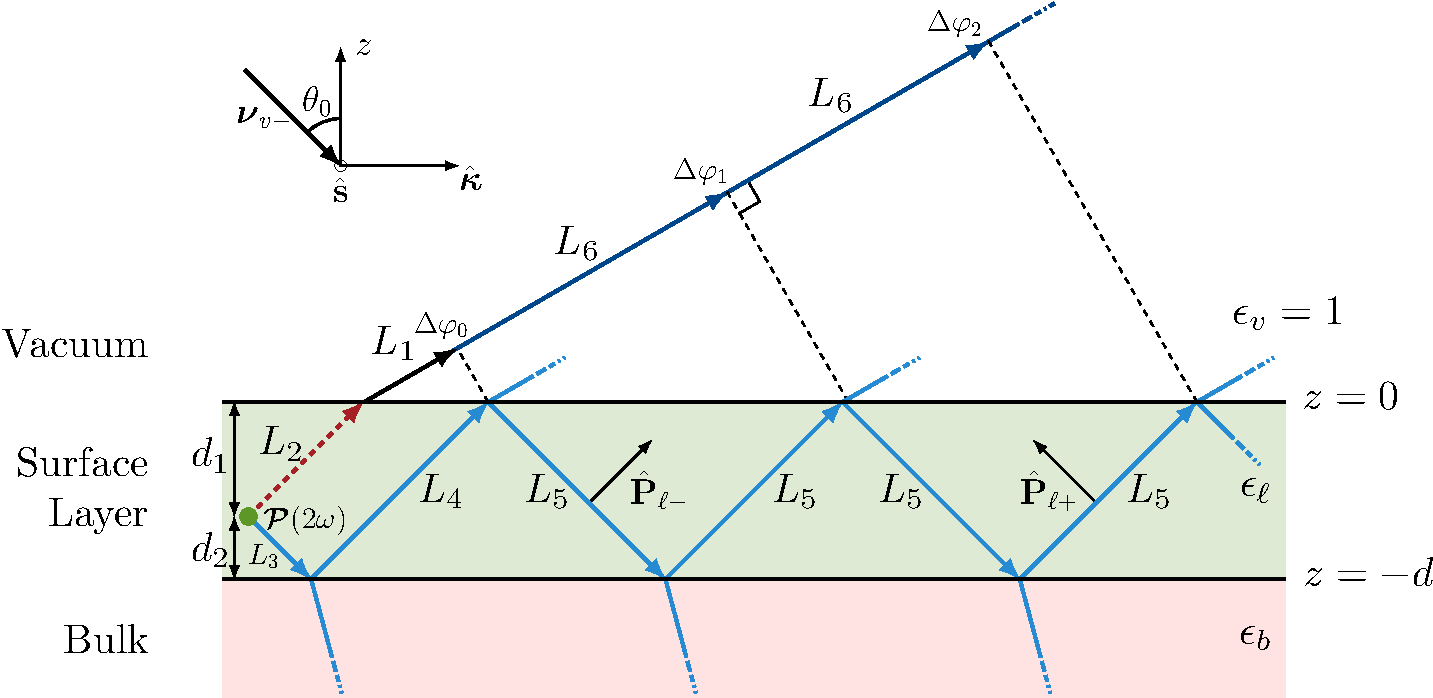
\includegraphics[width=0.48\textwidth]{fig1}
\caption{(Color online) Sketch of the three layer model for SHG. The vacuum
region ($v$) is on top with $\epsilon_{v}=1$; the layer $\ell$ of thickness $d =
d_{1} + d_{2}$, is characterized by $\epsilon_{\ell}(\omega)$, and it is where
the SH polarization sheet $\boldsymbol{\mathcal{P}}_{\ell}(2\omega)$ is located
at $z_{\ell} = d_{1}$. The bulk $b$ is described by $\epsilon_{b}(\omega)$. The
arrows point along the direction of propagation, and the $p$-polarization unit
vector, $\hat{\mathbf{P}}_{\ell -(+)}$, along the downward (upward) direction is
denoted with a thick arrow. The $s$-polarization unit vector $\hat{\mathbf{s}}$
points out of the page. The fundamental field $\mathbf{E}_v(\omega)$ is incident
from the vacuum side along the $\hat{\boldsymbol{\kappa}}z$-plane, with
$\theta_{0}$ being its angle of incidence and $\boldsymbol{\nu}_{v-}$ its wave
vector. $\Delta\varphi_{i}$ denotes the phase difference between the multiple
reflected beams and the first layer-vacuum transmitted beam, denoted by the
dashed-red arrow (of length $L_{2}$) followed by the solid black arrow (of
length $L_{1}$). The dotted lines in the vacuum region are perpendicular to the
beam extended from the solid black arrow (denoted by solid dark blue arrows of
length $L_{6}$).}
\label{fig:MR3layer2w}
\end{figure}

From Fig. \ref{fig:MR3layer2w}, we observe the propagation of the SH field as it
is refracted at the layer-vacuum interface ($\ell v$), and reflected multiple
times from the layer-bulk ($\ell b$) and layer-vacuum ($\ell v$) interfaces.
Thus, we can define
\begin{equation}\label{eq:r5}
\mathbf{T}^{\ell v}
= \hat{\mathbf{s}}T_{s}^{\ell v}\hat{\mathbf{s}} 
+ \hat{\mathbf{P}}_{v+}T_{p}^{\ell v} \hat{\mathbf{P}}_{\ell +}
\end{equation}
as the transmission tensor for the $\ell v$ interface,
\begin{equation}\label{eq:r6}
\mathbf{R}^{\ell b}
= \hat{\mathbf{s}}R_{s}^{\ell b}\hat{\mathbf{s}}
+ \hat{\mathbf{P}}_{\ell +}R_{p}^{\ell b} \hat{\mathbf{P}}_{\ell -}
\end{equation} 
as the reflection tensor for the $\ell b$ interface, and
\begin{equation}\label{eq:r6b}
\mathbf{R}^{\ell v}
= \hat{\mathbf{s}}R_{s}^{\ell v}\hat{\mathbf{s}}
+ \hat{\mathbf{P}}_{\ell -}R_{p}^{\ell v} \hat{\mathbf{P}}_{\ell +}
\end{equation} 
as the reflection tensor for the $\ell v$ interface. The Fresnel factors in
uppercase letters, $T^{ij}_{s,p}$ and $R^{ij}_{s,p}$, are evaluated at $2\omega$
from the following well known formulas \cite{jacksonbook}
\begin{equation}\label{eq:e.f1}
\begin{split}
t_{s}^{ij}(\omega) &=
\frac{2w_{i}(\omega)}{w_{i}(\omega) + w_{j}(\omega)},\\
t_{p}^{ij}(\omega) &=
\frac{2w_{i}(\omega)\sqrt{\epsilon_{i}(\omega)\epsilon_j(\omega)}}
     {w_{i}(\omega)\epsilon_{j}(\omega) + w_{j}(\omega)\epsilon_{i}(\omega)},\\
r_{s}^{ij}(\omega) &=
\frac{w_{i}(\omega) - w_{j}(\omega)}
     {w_{i}(\omega) + w_{j}(\omega)},\\
r_{p}^{ij}(\omega) &=
\frac{w_{i}(\omega)\epsilon_{j}(\omega) - w_{j}\epsilon_{i}(\omega)}
     {w_{i}(\omega)\epsilon_{j}(\omega) + w_{j}(\omega)\epsilon_{i}(\omega)}. 
\end{split}
\end{equation}
With these expressions, we easily derive the following useful relations,
\begin{equation}\label{eq:mf}
\begin{split}
1 + r^{\ell b}_{s} &= t^{\ell b}_{s},\\
1 + r^{\ell b}_{p} &= \frac{n_{b}}{n_{\ell}}t^{\ell b}_{p},\\
1 - r^{\ell b}_{p} &= \frac{n_{\ell}}{n_{b}}\frac{w_{b}}{w_{\ell}}
                      t^{\ell b}_{p},\\
t^{\ell v}_{p} &= \frac{w_{\ell}}{w_{v}}t^{v\ell}_{p},\\
t^{\ell v}_{s} &= \frac{w_{\ell}}{w_{v}}t^{v\ell}_{s}.
\end{split}
\end{equation}


%%%%%%%%%%%%%%%%%%%%%%%%%%%%%%%%%%%%%%%%%%%%%%%%%%%%%%%%%%%%%%%%%%%%%%%%%%%%%%%%

\subsection{Multiple SHG reflections}\label{sec:multiple2w}

The SH field $\mathbf{E}(2\omega)$ generated by the SH polarization
$\boldsymbol{\mathcal{P}}_{\ell}(2\omega)$ will radiate directly into the vacuum
and bulk, where it will be reflected back into the thin layer at the layer-bulk
interface; this beam will be transmitted and reflected multiple times, as shown
in Fig. \ref{fig:MR3layer2w}. As the two beams propagate, a phase difference
will develop between them according to
\begin{equation}\label{eq:m99}
\begin{split}
\Delta\varphi_{m} 
&= \tilde{\Omega}
\Big(
\big(L_{3} + L_{4} + 2mL_{5}\big)N_{\ell}\\
 &\hspace{14pt}- \big(L_{2}N_{\ell} + (L_{1} + mL_{6})N_{v}\big)
\Big)\\
&= \delta_{0} + m\delta\quad m=0,1,2,\ldots,
\end{split}
\end{equation}
where
\begin{equation}\label{eq:delta0}
\delta_{0} =
8\pi\left(\frac{d_{2}}{\lambda_{0}}\right)W_{\ell},
\end{equation}
and
\begin{equation}\label{eq:delta}
\delta = 8\pi
\left(\frac{d}{\lambda_{0}}\right)W_{\ell},
\end{equation}
where $\lambda_{0}$ is the wavelength of the fundamental field in vacuum,
$W_{\ell}$ is established in Eq. \eqref{eq:wavevector}, $d$ is the thickness of
layer $\ell$, and $d_{2}$ is the distance between
$\boldsymbol{\mathcal{P}}_{\ell}(2\omega)$ and the $\ell b$ interface (see Fig.
\ref{fig:MR3layer2w}). We see that $\delta_{0}$ is the phase difference of the
first and second transmitted beams, and $m\delta$ that of the first and third
($m = 1$), first and fourth ($m = 2$), and so on. Note that the thickness $d$ of
the layer $\ell$ enters through the phase $\delta$, and the position $d_{2}$ of
the nonlinear polarization $\mathbf{P}(\mathbf{r},t)$ (Eq. \eqref{eq:psheet})
enters through $\delta_{0}$. In particular, $d_{2}$ could be used as a variable
to study the effects of multiple reflections on the SSHG yield
$\mathcal{R}(2\omega)$.

To take into account the multiple reflections of the generated SH field in the
layer $\ell$, we proceed as follows. We include the algebra for the
$p$-polarized SH field, but the $s$-polarized field can be worked out
{following} the same steps. The $p$-polarized $\mathbf{E}_{\ell,p}(2\omega)$
field that is reflected multiple times is given by
\begin{widetext}
\begin{equation}\label{eq:E2wcomplete}
\begin{split}
\mathbf{E}_{\ell,p}(2\omega) 
&= E_{\ell,p+}(2\omega)\mathbf{T}^{\ell v}\cdot\hat{\mathbf{P}}_{\ell +}
 + E_{\ell,p-}(2\omega)\mathbf{T}^{\ell v}
\cdot\mathbf{R}^{\ell b}\cdot\hat{\mathbf{P}}_{\ell-}e^{i\Delta\varphi_{0}}
 + E_{\ell,p-}(2\omega)\mathbf{T}^{\ell v}
\cdot\mathbf{R}^{\ell b}\cdot\mathbf{R}^{\ell v}
\cdot\mathbf{R}^{\ell b}\cdot\hat{\mathbf{P}}_{\ell-}e^{i\Delta\varphi_{1}}
\\
&+ E_{\ell,p-}(2\omega)\mathbf{T}^{\ell v}
\cdot\mathbf{R}^{\ell b}\cdot\mathbf{R}^{\ell v}
\cdot\mathbf{R}^{\ell b}\cdot\mathbf{R}^{\ell v}
\cdot\mathbf{R}^{\ell b}\cdot\hat{\mathbf{P}}_{\ell-}e^{i\Delta\varphi_{2}}
+\cdots\\
&= E_{\ell,p+}(2\omega)\mathbf{T}^{\ell v}\cdot\hat{\mathbf{P}}_{\ell +}
+ E_{\ell,p-}(2\omega) \mathbf{T}^{\ell v}
\cdot\sum_{m=0}^\infty  
\big(
\mathbf{R}^{\ell b}\cdot\mathbf{R}^{\ell v} 
e^{i\delta}\Big)^m 
\cdot\mathbf{R}^{\ell b}\cdot\hat{\mathbf{P}}_{\ell-}e^{i\delta_{0}}.
\end{split}
\end{equation}
\end{widetext}
From Eqs. \eqref{eq:r5}-\eqref{eq:r6b}, it is easy to show that
\begin{equation*}\label{eq:m1}
\begin{split}
\mathbf{T}^{\ell v}\cdot
\Big(\mathbf{R}^{\ell b}\cdot\mathbf{R}^{\ell v}\Big)^{m}\cdot
\mathbf{R}^{\ell b}
&= \hat{\mathbf{s}}T^{\ell v}_{s}
  \Big(R^{\ell b}_{s}R^{\ell v}_{s}\Big)^{m}R^{\ell b}_{s}\hat{\mathbf{s}}\\
&+ \hat{\mathbf{P}}_{v+}T^{\ell v}_{p}\Big(R^{\ell b}_{p}R^{\ell v}_{p}\Big)^m 
  R^{\ell b}_{p} 
\hat{\mathbf{P}}_{\ell-},
\end{split}
\end{equation*}
then,
\begin{equation*}\label{eq:E2wreduced}
\begin{split}
\mathbf{E}_{\ell,p}&(2\omega) =\\
&\hat{\mathbf{P}}_{\ell +}T^{\ell v}_{p}
\Big(
E_{\ell,p+}(2\omega) +
\frac{R^{\ell b}_{p}e^{i\delta_{0}}}{1 + R^{v\ell}_{p}R^{\ell b}_{p}e^{i\delta}}
E_{\ell,p-}(2\omega) 
\Big),
\end{split}
\end{equation*}
where we used $R^{ij}_{s,p} = -R^{ji}_{s,p}$. Using Eq. \eqref{eq:solmaxwell}
and \eqref{eq:mf}, we can readily write
\begin{equation}\label{eq:mr8}
\mathbf{E}_{\ell,p}(2\omega) =
\frac{\gamma i\tilde{\Omega}}{W_{\ell}}\mathbf{H}_{\ell}\cdot
\boldsymbol{\mathcal{P}}_{\ell}(2\omega),
\end{equation}
where
\begin{equation}\label{eq:mr9}
\begin{split}
\mathbf{H}_{\ell}
= \frac{W_\ell}{W_v}
&\Big[
\hat{\mathbf{s}}\,T_{s}^{v\ell}
\left(1+ R^{M}_{s}\right)\hat{\mathbf{s}}\\
&+ \hat{\mathbf{P}}_{v+}T_{p}^{v\ell}
\left(\hat{\mathbf{P}}_{\ell +} + R^{M}_{p}\hat{\mathbf{P}}_{\ell -}\right)
\Big],
\end{split}
\end{equation}
and
\begin{equation}\label{m61}
R^{M}_{\mathrm{i}}\equiv
\frac{R^{\ell b}_{\mathrm{i}}e^{i\delta_{0}}}
     {1+R^{v\ell}_{\mathrm{i}} R^{\ell b}_{\mathrm{i}}e^{i\delta}},
     \quad \mathrm{i}=s,p
\end{equation}
defines the multiple ($M$) reflection coefficient. This coefficient depends on
the thickness $d$ of layer $\ell$, and most importantly, on the position $d_{2}$
of $\boldsymbol{\mathcal{P}}_{\ell}(2\omega)$ within this layer. The final
results will depend on both $d$ and $d_{2}$. However, using Eq.
\eqref{eq:delta0} we can also define an average $\bar{R}^{M}_{\mathrm{i}}$ as
\begin{equation}\label{eq:mcave}
\begin{split}
\bar{R}^{M}_{\mathrm{i}}&\equiv 
\frac{1}{d}\int_{0}^{d}
\frac{R^{\ell b}_{\mathrm{i}}e^{i(8\pi W_{\ell}/\lambda_{0})x}}
{1 + R^{v\ell}_{\mathrm{i}}R^{\ell b}_{\mathrm{i}}e^{i\delta}}\,dx\\
&= \frac{R^{\ell b}_{\mathrm{i}}e^{i\delta/2}}
{1 + R^{v\ell}_{\mathrm{i}}R^{\ell b}_{\mathrm{i}}e^{i\delta}}
\,\mathrm{sinc}(\delta/2)
\end{split}
\end{equation}
that only depends on $d$ through the $\delta$ term from Eq. \eqref{eq:delta}.

To connect with the work in Ref. \onlinecite{mizrahiJOSA88}, where
$\boldsymbol{\mathcal{P}}(2\omega)$ is located on top of the vacuum-surface
interface, and only the vacuum radiated beam and the first (and only) reflected
beam need be considered, we take $\ell = v$ and $d_{2} = 0$, then $T^{\ell v} =
1$, $R^{v\ell} = 0$ and $\delta_{0} = 0$, with which $R^{M}_{\mathrm{i}} =
R^{vb}_{\mathrm{i}}$. Thus, Eq. \eqref{eq:mr9} coincides with Eq. (3.8) of Ref.
\onlinecite{mizrahiJOSA88}.


%%%%%%%%%%%%%%%%%%%%%%%%%%%%%%%%%%%%%%%%%%%%%%%%%%%%%%%%%%%%%%%%%%%%%%%%%%%%%%%%

\subsection{Multiple Reflections for the Linear Field}\label{sec:multiple1w}

For a more complete formulation, we must also consider the multiple reflections
of the fundamental field $\mathbf{E}_{\ell}(\omega)$ inside the thin $\ell$
layer. In Fig. \ref{fig:MR3layer1w}, we present the situation where
$\mathbf{E}_{v}(\omega)$ impinges from the vacuum side with an angle of
incidence $\theta_{0}$. As the first transmitted beam is reflected multiple
times from the $\ell b$ and the $v\ell$ interfaces, it accumulates a phase
difference of $n\varphi$ ($n=1,2,3,\ldots$), where $\varphi$ given by
\begin{equation}\label{mphi}
\begin{split}
\varphi &= \frac{\omega}{c}(2L_{1}n_{\ell} - L_{2}n_{v})\\
&= 4\pi\left(\frac{d}{\lambda_{0}}\right)w_{\ell},
\end{split}
\end{equation}
where $n_{v} = 1$. Besides the equivalent of Eqs. \eqref{eq:r6} and
\eqref{eq:r6b} for $\omega$, we also need
\begin{equation}\label{eq:mvv}
\mathbf{t}^{v\ell}
= \hat{\mathbf{s}}t_{s}^{v\ell}\hat{\mathbf{s}} 
+ \hat{\mathbf{p}}_{\ell -}t_{p}^{v\ell}\hat{\mathbf{p}}_{v-},
\end{equation}
to write
\begin{widetext}
\begin{equation}\label{eq:mcvew}
\begin{split}
\mathbf{E}_\ell(\omega)
&= E_{0}
\Big[
\mathbf{t}^{v\ell} + \mathbf{r}^{\ell b}\cdot\mathbf{t}^{v\ell}e^{i\varphi}
 + \mathbf{r}^{\ell b}\cdot\mathbf{r}^{\ell v}\cdot
   \mathbf{r}^{\ell b}\cdot\mathbf{t}^{v\ell} e^{i2\varphi}
 + \mathbf{r}^{\ell b}\cdot\mathbf{r}^{\ell v}\cdot
   \mathbf{r}^{\ell b}\cdot\mathbf{r}^{\ell v}\cdot
   \mathbf{r}^{\ell b}\cdot\mathbf{t}^{v\ell} e^{i3\varphi}
 + \cdots
\Big]\cdot\hat{\mathbf{e}}^{\mathrm{i}}\\
&= E_{0}
\Big[
1 + \Big(1 + \mathbf{r}^{\ell b}\cdot\mathbf{r}^{\ell v}e^{i\varphi}
+ (\mathbf{r}^{\ell b}\cdot\mathbf{r}^{\ell v})^2e^{i2\varphi}+\cdots\Big)\cdot
\mathbf{r}^{\ell b}e^{i\varphi}
\Big]
\cdot\mathbf{t}^{v\ell}\cdot\hat{\mathbf{e}}^{\mathrm{i}}\\
&= E_{0}
\Big[
\hat{\mathbf{s}} t^{v\ell}_{s}(1+r^{M}_{s})\hat{\mathbf{s}} 
+ t^{v\ell}_{p}
\left(\hat{\mathbf{p}}_{\ell-}+\hat{\mathbf{p}}_{\ell+}r^{M}_{p}\right)
\hat{\mathbf{p}}_{v-}
\Big]\cdot\hat{\mathbf{e}}^{\mathrm{i}},
\end{split}
\end{equation}
\end{widetext}
where $E_{0}$ is the intensity of the fundamental field, and
$\hat{\mathbf{e}}^{\mathrm{i}}$ is the unit vector of the incoming polarization,
with $\mathrm{i} = s,p$, and then, $\hat{\mathbf{e}}^{s}=\hat{\mathbf{s}}$ and
$\hat{\mathbf{e}}^{p}=\hat{\mathbf{p}}_{v-}$. Also,
\begin{equation}\label{mvrm}
r^{M}_{\mathrm{i}} \equiv
\frac{r^{\ell b}_{\mathrm{i}}e^{i\varphi}}{1+r^{v\ell}_{\mathrm{i}}
r^{\ell b}_{\mathrm{i}}e^{i\varphi}}, \quad \mathrm{i}=s,p.
\end{equation}
$r^{M}_{\mathrm{i}}$ is defined as the multiple (M) reflection coefficient for
the fundamental field. We define $\mathbf{E}^{\mathrm{i}}_{\ell}(\omega)\equiv
E_{0}\mathbf{e}^{\omega,\mathrm{i}}_{\ell}$ ($\mathrm{i}=s,p$), where
\begin{equation}\label{eq:mcvew2}
\mathbf{e}^{\omega,\mathrm{i}}_\ell 
= \Big[\hat{\mathbf{s}} t^{v\ell}_s(1+r^M_s)\hat{\mathbf{s}} 
+ t^{v\ell}_p\left(\hat{\mathbf{p}}_{\ell-}+\hat{\mathbf{p}}_{\ell+}r^{M}_p 
\right)\hat{\mathbf{p}}_{v-}
\Big]\cdot\hat{\mathbf{e}}^{\mathrm{i}},
\end{equation}
and using Eq. \eqref{eq:r4}, we obtain that
\begin{equation}\label{eq:mcvep}
\mathbf{e}^{\omega,p}_{\ell}=\frac{t^{v\ell}_{p}}{n_{\ell}}
\left( 
  r^{M+}_{p}\sin\theta_{0}\hat{\mathbf{z}}
+ r^{M-}_{p}w_{\ell}\hat{\boldsymbol{\kappa}}
\right)
\end{equation} 
for $p$-input polarization with $\hat{\mathbf{e}}^{\mathrm{i}} =
\hat{\mathbf{p}}_{v-}$, and
\begin{equation}\label{eq:mcves}
\mathbf{e}^{\omega,s}_\ell=t^{v\ell}_{s}r^{M+}_{s}\hat{\mathbf{s}}
\end{equation}
for $s$-input polarization with $\hat{\mathbf{e}}^{\mathrm{i}} =
\hat{\mathbf{s}}$, where
\begin{equation}\label{eq:mvc}
r^{M\pm}_{\mathrm{i}} = 1\pm r^{M}_{\mathrm{i}},\quad \mathrm{i} = s,p.
\end{equation}

\begin{figure}[t]
\centering 
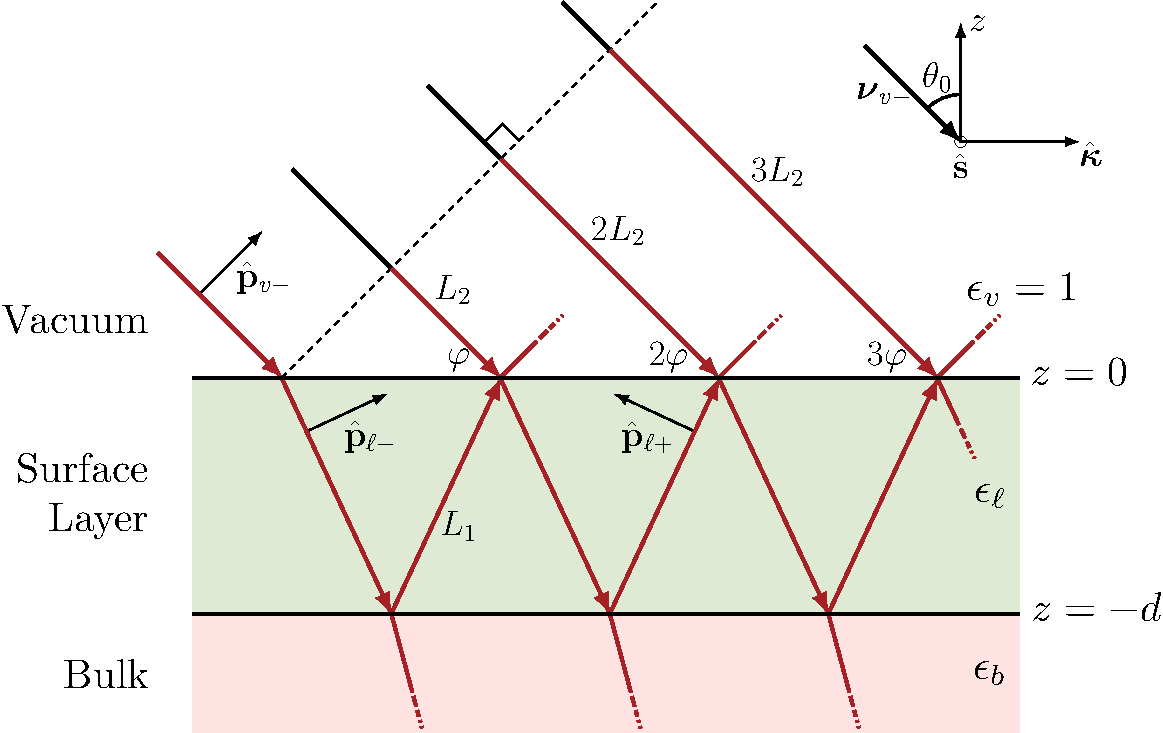
\includegraphics[width=0.48\textwidth]{fig2}
\caption{(Color online) Sketch for the multiple reflected fundamental field
$\mathbf{E}_\ell(\omega)$, which impinges from the vacuum side along the
$\hat{\boldsymbol{\kappa}}z$-plane. $\theta_{0}$ and $\boldsymbol{\nu}_{v-}$ are
the angle of incidence and wave vector, respectively. The arrows point along the
direction of propagation. The $p$-polarization unit vectors
$\hat{\mathbf{p}}_{\beta\pm}$, point along the downward $(-)$ or upward $(+)$
directions and are denoted with black arrows, where $\beta = v$ or $\ell$. The
$s$-polarization unit vector $\hat{\mathbf{s}}$ points out of the page.
$(1,2,3,\ldots)\varphi$ denotes the phase difference for the multiple reflected
beams with respect to the incident field, where the dotted line is perpendicular
to this beam.}
\label{fig:MR3layer1w}
\end{figure}


%%%%%%%%%%%%%%%%%%%%%%%%%%%%%%%%%%%%%%%%%%%%%%%%%%%%%%%%%%%%%%%%%%%%%%%%%%%%%%%%

\subsection{The SSHG yield}

The magnitude of the radiated field is given by $E(2\omega) =
\hat{\mathbf{e}}^{\mathrm{F}}\cdot\mathbf{E}_{\ell}(2\omega)$, where
$\hat{\mathbf{e}}^{\mathrm{F}}$ is the unit vector of the final, $S$ or $P$ SH
polarization with $\mathrm{F} = S,P$, where
$\hat{\mathbf{e}}^S=\hat{\mathbf{s}}$ and
$\hat{\mathbf{e}}^P=\hat{\mathbf{P}}_{v+}$. We expand the rightmost term in
parenthesis of Eq. \eqref{eq:mr9} as
\begin{equation*}
\begin{split}
\hat{\mathbf{P}}_{\ell +} + R^{M}_{p}\hat{\mathbf{P}}_{\ell -}
&= \frac{\sin\theta_{0}\hat{\mathbf{z}} - W_{\ell}\hat{\boldsymbol{\kappa}}}
        {N_{\ell}}
 + R^{M}_{p}
   \frac{\sin\theta_{0}\hat{\mathbf{z}} + W_{\ell}\hat{\boldsymbol{\kappa}}}
        {N_{\ell}}\\
&= \frac{1}{N_{\ell}}
\left(
\sin\theta_{0}R^{M+}_{p}\hat{\mathbf{z}}
- W_{\ell}R^{M-}_{p}\hat{\boldsymbol{\kappa}}
\right),
\end{split}
\end{equation*}
where
\begin{equation}\label{eq:rm}
R^{M\pm}_{\mathrm{i}}\equiv 1 \pm R^{M}_{\mathrm{i}}, \quad \mathrm{i}=s,p.
\end{equation}
Using Eq. \eqref{eq:mf}, we write Eq. \eqref{eq:mr8} as
\begin{equation}\label{eq:r10}
\begin{split}
E(2\omega) &= \frac{2\gamma i\omega}{cW_\ell}
\hat{\mathbf{e}}^{\mathrm{F}}\cdot\mathbf{H}_{\ell}\cdot
\boldsymbol{\mathcal{P}}_{\ell}(2\omega)\\
&= \frac{2\gamma i\omega}{cW_{v}}
\mathbf{e}^{\,2\omega,\mathrm{F}}_{\ell}\cdot
\boldsymbol{\mathcal{P}}_{\ell}(2\omega),
\end{split}
\end{equation}
where
\begin{align}\label{eq:r12mm}
\mathbf{e}^{2\omega,\mathrm{F}}_{\ell} &= 
\hat{\mathbf{e}}^{\mathrm{F}}\cdot 
\Bigg[
\hat{\mathbf{s}}T_{s}^{v\ell}R^{M+}_{s}\hat{\mathbf{s}}\\
&\hspace{4em}+ \hat{\mathbf{P}}_{v+}
\frac{T^{v\ell}_{p}}
     {N_{\ell}}
\left(
\sin\theta_{0}R^{M+}_{p}\hat{\mathbf{z}}
- W_{\ell}R^{M-}_{p}\hat{\boldsymbol{\kappa}}
\right) 
\Bigg].\nonumber
\end{align}  
Replacing $\mathbf{E}_\ell(\omega)\to E_0\mathbf{e}^{\omega,\mathrm{i}}_\ell$
in Eq. \eqref{eq:tres}, we obtain that
\begin{equation}\label{eq:m4}
\boldsymbol{\mathcal{P}}_{\ell}(2\omega) = 
\left\{
\begin{array}{cc}  
E^{2}_{0}\,
\boldsymbol{\chi}_{\mathrm{surface}}:\mathbf{e}^{\omega,\mathrm{i}}_{\ell}
                  \mathbf{e}^{\omega,\mathrm{i}}_{\ell}
& \text{(CGS units)}\\\\
\epsilon_{0}E^{2}_{0}\,
\boldsymbol{\chi}_{\mathrm{surface}}:\mathbf{e}^{\omega,\mathrm{i}}_{\ell}
                  \mathbf{e}^{\omega,\mathrm{i}}_{\ell}
& \text{(MKS units)}\\
\end{array}
\right.,
\end{equation}
where $\mathbf{e}^{\omega,\mathrm{i}}_{\ell}$ is given by Eq. \eqref{eq:mcvew2},
and thus Eq. \eqref{eq:r10} reduces to ($W_{v} = \cos\theta_{0}$)
\begin{equation}\label{eq:mr10}
E_{\ell}(2\omega) 
= \frac{2\eta i \omega}{c\cos\theta_{0}}
\mathbf{e}^{2\omega,\mathrm{F}}_{\ell}\cdot
\boldsymbol{\chi}_{\mathrm{surface}}:\mathbf{e}^{\omega,\mathrm{i}}_{\ell}
                  \mathbf{e}^{\omega,\mathrm{i}}_{\ell},
\end{equation}
where $\eta = 2\pi$ in CGS units and $\eta = 1/2$ in MKS units. For ease of
notation, we define
\begin{align}\label{eq:mc0}
\Upsilon_{\mathrm{iF}}
\equiv 
\mathbf{e}^{2\omega,\mathrm{F}}_{\ell}\cdot
\boldsymbol{\chi}_{\mathrm{surface}}:\mathbf{e}^{\omega,\mathrm{i}}_{\ell}
                  \mathbf{e}^{\omega,\mathrm{i}}_{\ell},
\end{align}
where i stands for the incoming polarization of the fundamental electric field
given by $\hat{\mathbf{e}}^{\mathrm{i}}$ in Eq. \eqref{eq:mcvew2}, and F for the
outgoing polarization of the SH electric field given by
$\hat{\mathbf{e}}^{\mathrm{F}}$ in Eq. \eqref{eq:r12mm}. We purposely omit the
full $\boldsymbol{\chi}(-2\omega;\omega,\omega)$ notation, and will do so from
this point on.

From Eqs. \eqref{eq:rintensities} and \eqref{eq:intensity} we obtain that in CGS
units ($\eta = 2\pi$),
\begin{align}\label{eq:r01}
\vert E(2\omega)\vert^{2} &=
\vert E_{0}\vert^{4}\frac{16\pi^{2}\omega^{2}}{c^{2}W^2_{v}}
\vert\Upsilon_{\mathrm{iF}}\vert^{2}\nonumber\\
%%%%%%%%%%%%%%%%%%%%%%%%%%%%%%%%%%%%%%%%%%%%%%%%%%%%%
\frac{c}{2\pi}\vert\sqrt{N_{v}}E(2\omega)\vert^{2} &=
\frac{32\pi^{3}\omega^{2}}{c^{3}\cos^2\theta_{0}}
\left\vert\frac{\sqrt{N_{v}}}{n^{2}_{\ell}}\Upsilon_{\mathrm{iF}}\right\vert^{2} 
\left(\frac{c}{2\pi}\vert\sqrt{n_{\ell}}E_{0}\vert^{2}\right)^{2}\nonumber\\ 
%%%%%%%%%%%%%%%%%%%%%%%%%%%%%%%%%%%%%%%%%%%%%%%%%%%%%
I(2\omega) &=
\frac{32\pi^{3}\omega^{2}}{c^{3}\cos^2\theta_{0}}
\left\vert\frac{\sqrt{N_{v}}}{n^{2}_{\ell}}\Upsilon_{\mathrm{iF}}\right\vert^{2}
I^{2}(\omega)\nonumber\\
%%%%%%%%%%%%%%%%%%%%%%%%%%%%%%%%%%%%%%%%%%%%%%%%%%%%%
\mathcal{R}_{\mathrm{iF}}(2\omega) &=
\frac{32\pi^{3}\omega^{2}}{c^{3}\cos^2\theta_{0}}
\left\vert\frac{1}{n_{\ell}}\Upsilon_{\mathrm{iF}}\right\vert^{2},
\end{align} 
and in MKS units ($\eta=1/2$),
\begin{align}\label{r01m}
\vert E(2\omega)\vert^{2} &=
\vert E_{0}\vert^{4}\frac{\omega^{2}}{c^{2}W^{2}_{v}}\nonumber\\
%%%%%%%%%%%%%%%%%%%%%%%%%%%%%%%%%%%%%%%%%%%%%%%%%%%%%
2\epsilon_{0}c|\sqrt{N_{v}}E(2\omega)|^{2} &=
\frac{2\epsilon_{0}\omega^{2}}{c\cos^{2}\theta_{0}}
\left\vert\frac{\sqrt{N_{v}}}{n^{2}_{\ell}}\Upsilon_{\mathrm{iF}}\right\vert^{2} 
\frac{1}{4\epsilon^{2}_0c^{2}}
\left(2\epsilon_{0}c\vert\sqrt{n_{\ell}}E_{0}\vert^{2}\right)^{2}\nonumber\\
%%%%%%%%%%%%%%%%%%%%%%%%%%%%%%%%%%%%%%%%%%%%%%%%%%%%%
I(2\omega) &= 
\frac{\omega^{2}}{2\epsilon_{0}c^3\cos^{2}\theta_{0}}
\left\vert\frac{\sqrt{N_{v}}}{n^{2}_{\ell}}\Upsilon_{\mathrm{iF}}\right\vert^{2}
I^{2}(\omega)\nonumber\\
%%%%%%%%%%%%%%%%%%%%%%%%%%%%%%%%%%%%%%%%%%%%%%%%%%%%%
\mathcal{R}_{\mathrm{iF}}(2\omega) &=
\frac{\omega^{2}}{2\epsilon_{0}c^3\cos^{2}\theta_{0}}
\left\vert  \frac{1}{n_{\ell}}\Upsilon_{\mathrm{iF}}\right\vert^{2}.
\end{align}
Finally, we condense these results and establish the SSHG yield as
\begin{equation}\label{eq:mc6}
\mathcal{R}_{\mathrm{iF}}(2\omega) 
\left\{
\begin{array}{ r c } 
\frac{32\pi^{3}\omega^{2}}{c^{3}\cos^{2}\theta_{0}}
\left\vert\frac{1}{n_{\ell}}\Upsilon_{\mathrm{iF}}\right\vert^{2} 
& \text{(CGS units)} \\\\
\frac{\omega^{2}}{2\epsilon_{0}c^3\cos^{2}\theta_{0}}
\left\vert\frac{1}{n_{\ell}}\Upsilon_{\mathrm{iF}}\right\vert^{2} 
& \text{(MKS units)} 
\end{array}
\right.,
\end{equation}
where $N_{v} = 1$ and $W_{v} = \cos\theta_{0}$. We mention that
$\boldsymbol{\chi}_{\mathrm{surface}}$ is given in m$^{2}$/V in the MKS unit
system since it is a surface second order nonlinear susceptibility. In this
system of units, $\mathcal{R}_{\mathrm{iF}}$ is in m$^{2}$/W.


%%%%%%%%%%%%%%%%%%%%%%%%%%%%%%%%%%%%%%%%%%%%%%%%%%%%%%%%%%%%%%%%%%%%%%%%%%%%%%%%
%%%%%%%%%%%%%%%%%%%%%%%%%%%%%%%%%%%%%%%%%%%%%%%%%%%%%%%%%%%%%%%%%%%%%%%%%%%%%%%%

\section{\texorpdfstring{$\mathcal{R}_{\mathrm{iF}}$}{R} for Different
Polarization Cases}\label{sec:rcases}

We now have everything needed to derive explicit expressions for
$\mathcal{R}_{\mathrm{iF}}$, Eq. \eqref{eq:mc6}, for the most commonly used
polarizations of incoming and outgoing fields (iF=$pP$, $pS$, $sP$, and $sS$).
For this, we must expand $\Upsilon_{\mathrm{iF}}$ from Eq. \eqref{eq:mc0} for
each case. By substituting Eqs. \eqref{eq:mc1} and \eqref{eq:mmc2} into Eq.
\eqref{eq:r12mm}, we obtain
\begin{equation}\label{eq:e2wpmr}
\begin{split}
\mathbf{e}^{2\omega,P}_{\ell} &=
\frac{T^{v\ell}_{p}}{N_{\ell}}
\big(
  \sin\theta_{0}R^{M+}_{p}\hat{\mathbf{z}}\\
&- W_{\ell}R^{M-}_{p}\cos\phi\hat{\mathbf{x}}
- W_{\ell}R^{M-}_{p}\sin\phi\hat{\mathbf{y}}
\big),
\end{split}
\end{equation}
for $P$ $(\hat{\mathbf{e}}^{\mathrm{F}} = \hat{\mathbf{P}}_{v+})$ outgoing
polarization, and
\begin{equation}\label{eq:e2wsmr}
\mathbf{e}^{2\omega,S}_{\ell} =
T_{s}^{v\ell}R^{M+}_{s}
\left(
- \sin\phi\hat{\mathbf{x}}
+ \cos\phi\hat{\mathbf{y}}
\right).
\end{equation}
for $S$ $(\hat{\mathbf{e}}^{\mathrm{F}} = \hat{\mathbf{s}})$ outgoing
polarization.

Following a similar procedure, we use Eqs. \eqref{eq:mc1} and \eqref{eq:mmc2}
with Eq. \eqref{eq:mcvep}, and obtain
\begin{widetext}
\begin{equation}\label{eq:ewewpmr}
\begin{split}
\mathbf{e}^{\omega,\mathrm{p}}_{\ell}\mathbf{e}^{\omega,\mathrm{p}}_{\ell} =
\left(\frac{t^{v\ell}_{p}}{n_{\ell}}\right)^{2}
\bigg(
 &\big(r^{M-}_{p}\big)^{2}w^{2}_{\ell}\cos^{2}\phi
  \hat{\mathbf{x}}\hat{\mathbf{x}}
+ 2\big(r^{M-}_{p}\big)^{2}w^{2}_{\ell}\sin\phi\cos\phi
  \hat{\mathbf{x}}\hat{\mathbf{y}}
+ 2r^{M+}_{p}r^{M-}_{p}w_{\ell}\sin\theta_{0}\cos\phi
  \hat{\mathbf{x}}\hat{\mathbf{z}}\\
&+ \big(r^{M-}_{p}\big)^{2}w^{2}_{\ell}\sin^{2}\phi
  \hat{\mathbf{y}}\hat{\mathbf{y}}
+ 2r^{M+}_{p}r^{M-}_{p}w_{\ell}\sin\theta_{0}\sin\phi
  \hat{\mathbf{y}}\hat{\mathbf{z}}
+ \big(r^{M+}_{p}\big)^{2}\sin^{2}\theta_{0}
   \hat{\mathbf{z}}\hat{\mathbf{z}}
\bigg),
\end{split}
\end{equation}
\end{widetext}
for $p$ incoming polarization $(\hat{\mathbf{e}}^{\mathrm{i}} =
\hat{\mathbf{p}}_{v-})$, and with Eq. \eqref{eq:mcves},
\begin{equation}\label{eq:ewewsmr}
\mathbf{e}^{\omega,\mathrm{s}}_{\ell}\mathbf{e}^{\omega,\mathrm{s}}_{\ell}
= \left(t^{v\ell}_{s}r^{M+}_{s}\right)^{2}
\big(
  \sin^{2}\phi\hat{\mathbf{x}}\hat{\mathbf{x}}
 + \cos^{2}\phi\hat{\mathbf{y}}\hat{\mathbf{y}}
 - 2\sin\phi\cos\phi\hat{\mathbf{x}}\hat{\mathbf{y}}
\big).
\end{equation}
for $s$ incoming polarization $(\hat{\mathbf{e}}^{\mathrm{i}} =
\hat{\mathbf{s}})$. We have summarized the combination of equations needed to
derive the expressions for all four polarization cases of
$\mathcal{R}_{\mathrm{iF}}$ in Table \ref{tab:summary}. In the following
subsections we will derive the explicit expressions for $\Upsilon_{\mathrm{iF}}$
for the most general case where the surface has no symmetry. We will then
develop these expressions for particular cases of the most commonly investigated
surfaces, the (111), (001) and (110) crystallographic faces. For ease of
{\color{red}
notation, we split $\Upsilon_{\mathrm{iF}}$ as
\begin{equation}\label{eq:mc25}
\Upsilon_{\mathrm{iF}} = \Gamma_{\mathrm{iF}}\,r_{\mathrm{iF}},
\end{equation}
and omit the ``surface''subscript for the $\chi^{\mathrm{abc}}$ components. A
full, step-by-step derivation for all of these expressions can be found in Ref.
\onlinecite{andersonPHD16}, with and without the effects of multiple
reflections.
}

\begin{table}[t]
\caption{(Color online) Polarization unit vectors for
$\hat{\mathbf{e}}^{\mathrm{F}}$ and $\hat{\mathbf{e}}^{\mathrm{i}}$, and
equations describing $\mathbf{e}^{2\omega,\mathrm{F}}_{\ell}$ and
$\mathbf{e}^{\omega,\mathrm{i}}_{\ell}\mathbf{e}^{\omega,\mathrm{i}}_{\ell}$ for
each polarization case.}
\label{tab:summary}
\centering
\begin{tabular}{| c | l | l | c | c |}
\hline
Case               & $\hat{\mathbf{e}}^{\mathrm{F}}$
                   & $\hat{\mathbf{e}}^{\mathrm{i}}$
                   & $\mathbf{e}^{2\omega,\mathrm{F}}_{\ell}$
                   & $\mathbf{e}^{\omega,\mathrm{i}}_{\ell}
                      \mathbf{e}^{\omega,\mathrm{i}}_{\ell}$ \\
\hline
$\mathcal{R}_{pP}$ & $\hat{\mathbf{P}}_{v+}$
                   & $\hat{\mathbf{p}}_{v-}$
                   &  Eq. \eqref{eq:e2wpmr} & Eq. \eqref{eq:ewewpmr} \\
$\mathcal{R}_{pS}$ & $\hat{\mathbf{S}}$
                   & $\hat{\mathbf{p}}_{v-}$
                   &  Eq. \eqref{eq:e2wsmr} & Eq. \eqref{eq:ewewpmr} \\
$\mathcal{R}_{sP}$ & $\hat{\mathbf{P}}_{v+}$
                   & $\hat{\mathbf{s}}$
                   &  Eq. \eqref{eq:e2wpmr} & Eq. \eqref{eq:ewewsmr} \\
$\mathcal{R}_{sS}$ & $\hat{\mathbf{S}}$
                   & $\hat{\mathbf{s}}$
                   &  Eq. \eqref{eq:e2wsmr} & Eq. \eqref{eq:ewewsmr} \\
\hline
\end{tabular}
\end{table}

{\color{red} Many expressions can be greatly simplified by introducing a matrix
representation for $\boldsymbol{\chi}$. Disregarding all symmetry relations, we
have
\begin{equation}
\boldsymbol{\chi} =
\begin{pmatrix}
\chi^{xxx}&\chi^{xyy}&\chi^{xzz} &|& \chi^{xyz}&\chi^{xxz}&\chi^{xxy} \\[3pt]
\chi^{yxx}&\chi^{yyy}&\chi^{yzz} &|& \chi^{yyz}&\chi^{yxz}&\chi^{yxy} \\[3pt]
\chi^{zxx}&\chi^{zyy}&\chi^{zzz} &|& \chi^{zyz}&\chi^{zxz}&\chi^{zxy}
\end{pmatrix}
,
\end{equation}
where all 18 independent components are accounted for, recalling that
$\chi^{\mathrm{abc}} = \chi^{\mathrm{acb}}$ for SHG. Notice that the left hand
block contains the components of $\chi^{\mathrm{abc}}$ where $b = c$, and the
right hand block those where $b \neq c$. As mentioned above, we are interested
in the (111), (110) and (001) crystallographic faces, that belong to the
$C_{3v}$, $C_{2v}$, and $C_{4v}$ symmetry groups, respectively. For the (111)
surface, we choose the $x$ and $y$ axes along the [$11\bar{2}$] and
[$1\bar{1}0$] directions, respectively. For the (110) and (001), we consider the
$y$ axis perpendicular to the plane of symmetry.\cite{sipePRB87} These are
represented in matrix form as
\begin{equation}\label{eq:111matrix}
\boldsymbol{\chi}^{(111)} =
\begin{pmatrix}
\chi^{xxx}&-\chi^{xxx}&    0      &|&     0     &\chi^{xxz}&     0     \\[3pt]
     0    &      0    &    0      &|& \chi^{xxz}&     0   &-\chi^{xxx}\\[3pt]
\chi^{zxx}& \chi^{zxx}&\chi^{zzz} &|&     0     &     0    &     0 
\end{pmatrix}
,
\end{equation}
\begin{equation}\label{eq:110matrix}
\boldsymbol{\chi}^{(110)} =
\begin{pmatrix}
     0    &     0    &     0     &|&      0    &\chi^{xxz}&     0     \\[3pt]
     0    &     0    &     0     &|& \chi^{yyz}&     0    &     0     \\[3pt]
\chi^{zxx}&\chi^{zyy}&\chi^{zzz} &|&      0    &     0    &     0
\end{pmatrix}
,
\end{equation}
and
\begin{equation}\label{eq:001matrix}
\boldsymbol{\chi}^{(001)} =
\begin{pmatrix}
     0    &     0    &     0     &|&      0    &\chi^{xxz}&     0     \\[3pt]
     0    &     0    &     0     &|& \chi^{xxz}&     0    &     0     \\[3pt]
\chi^{zxx}&\chi^{zxx}&\chi^{zzz} &|&      0    &     0    &     0
\end{pmatrix}
.
\end{equation}
In general, $\boldsymbol{\chi}^{(111)}\ne \boldsymbol{\chi}^{(110)} \ne 
\boldsymbol{\chi}^{(001)}$.
}

% \begin{table}[b]
% \caption{(Color online) Nonzero components of $\boldsymbol{\chi}$ for the (111),
% (110) and (001) crystallographic faces, belonging to the $C_{3v}$, $C_{2v}$, and
% $C_{4v}$ symmetry groups, respectively. For the (111) surface, we choose the
% $x$ and $y$ axes along the [$11\bar{2}$] and [$1\bar{1}0$] directions,
% respectively. For the (110) and (001), we consider the $y$ axis perpendicular to
% the plane of symmetry.\cite{sipePRB87} In general $\boldsymbol{\chi}^{(111)}\ne
% \boldsymbol{\chi}^{(110)} \ne \boldsymbol{\chi}^{(001)}$.}
% \label{tab:chis}
% \centering
% \begin{tabular}{| c | c | c |}
% \hline 
% (111)-$C_{3v}$          & (110)-$C_{2v}$            & (001)-$C_{4v}$ \\
% \hline 
% $\chi^{zzz}$            & $\chi^{zzz}$              & $\chi^{zzz}$\\
% $\chi^{zxx}=\chi^{zyy}$ & $\chi^{zxx}\ne\chi^{zyy}$ & $\chi^{zxx}=\chi^{zyy}$\\
% $\chi^{xxz}=\chi^{yyz}$ & $\chi^{xxz}\ne\chi^{yyz}$ & $\chi^{xxz}=\chi^{yyz}$\\
% $\chi^{xxx}=-\chi^{xyy}=-\chi^{yxy}$ &              &  \\
% \hline 
% \end{tabular}
% \end{table}


%%%%%%%%%%%%%%%%%%%%%%%%%%%%%%%%%%%%%%%%%%%%%%%%%%%%%%%%%%%%%%%%%%%%%%%%%%%%%%%%

\subsection{\texorpdfstring{$\mathcal{R}_{pP}$ ($p$-in, $P$-out)}
{RpP (p-in, P-out)}}
\label{sec:RpP} 

Per Table \ref{tab:summary}, $\mathcal{R}_{pP}$ requires Eqs. \eqref{eq:e2wpmr}
and \eqref{eq:ewewpmr}. After some algebra, we obtain that
\begin{equation}\label{eq:mc78}
\Gamma_{pP} =
\frac{T^{v\ell}_{p}}{N_{\ell}}
\left(\frac{t^{v\ell}_{p}}{n_{\ell}}\right)^{2}
,
\end{equation}
and
% \begin{widetext}
% \begin{equation}
% \begin{split}
% r_{pP} =
% &-R^{M-}_{p}\left(r^{M-}_{p}\right)^{2}w^{2}_{\ell}W_{\ell}\cos^{3}\phi
% \chi^{xxx}
%  -2R^{M-}_{p}\left(r^{M-}_{p}\right)^{2}w^{2}_{\ell}W_{\ell}\sin\phi\cos^{2}\phi
% \chi^{xxy}\\
% &-2R^{M-}_{p}r^{M+}_{p}r^{M-}_{p}w_{\ell}W_{\ell}\sin\theta_{0}\cos^{2}\phi
% \chi^{xxz}
%  -R^{M-}_{p}\left(r^{M-}_{p}\right)^{2}w^{2}_{\ell}W_{\ell}\sin^{2}\phi\cos\phi
% \chi^{xyy}\\
% &-2R^{M-}_{p}r^{M+}_{p}r^{M-}_{p}w_{\ell}W_{\ell}\sin\theta_{0}\sin\phi\cos\phi
% \chi^{xzy}
%  -R^{M-}_{p}\left(r^{M+}_{p}\right)^{2}W_{\ell}\sin^{2}\theta_{0}\cos\phi
% \chi^{xzz}\\
% %%%%%%%%%%%%%%%%%%%%%%%%%%%%%%%%%%%%%%%%%%%%%%%%%%%%%%%%%%%%
% &-R^{M-}_{p}\left(r^{M-}_{p}\right)^{2}w^{2}_{\ell}W_{\ell}\sin\phi\cos^{2}\phi
% \chi^{yxx}
%  -2R^{M-}_{p}\left(r^{M-}_{p}\right)^{2}w^{2}_{\ell}W_{\ell}\sin^{2}\phi\cos\phi
% \chi^{yxy}\\
% &-2R^{M-}_{p}r^{M+}_{p}r^{M-}_{p}w_{\ell}W_{\ell}\sin\theta_{0}\sin\phi\cos\phi
% \chi^{yxz}
%  -R^{M-}_{p}\left(r^{M-}_{p}\right)^{2}w^{2}_{\ell}W_{\ell}\sin^{3}\phi
% \chi^{yyy}\\
% &-2R^{M-}_{p}r^{M+}_{p}r^{M-}_{p}w_{\ell}W_{\ell}\sin\theta_{0}\sin^{2}\phi
% \chi^{yyz}
%  -R^{M-}_{p}\left(r^{M+}_{p}\right)^{2}W_{\ell}\sin^{2}\theta_{0}\sin\phi
% \chi^{yzz}\\
% %%%%%%%%%%%%%%%%%%%%%%%%%%%%%%%%%%%%%%%%%%%%%%%%%%%%%%%%%%%%
% &+R^{M+}_{p}\left(r^{M-}_{p}\right)^{2}w^{2}_{\ell}\sin\theta_{0}\cos^{2}\phi
% \chi^{zxx}
%  +2R^{M+}_{p}r^{M+}_{p}r^{M-}_{p}w_{\ell}\sin^{2}\theta_{0}\cos\phi
% \chi^{zxz}\\
% &+2R^{M+}_{p}\left(r^{M-}_{p}\right)^{2}w^{2}_{\ell}\sin\theta_{0}\sin\phi
% \cos\phi\chi^{zxy}
%  +R^{M+}_{p}\left(r^{M-}_{p}\right)^{2}w^{2}_{\ell}\sin\theta_{0}\sin^{2}\phi
% \chi^{zyy}\\
% &+2R^{M+}_{p}r^{M+}_{p}r^{M-}_{p}w_{\ell}\sin^{2}\theta_{0}\sin\phi
% \chi^{zzy}
%  +R^{M+}_{p}\left(r^{M+}_{p}\right)^{2}\sin^{3}\theta_{0}
% \chi^{zzz},
% \end{split}
% \end{equation}
% \end{widetext}
{\color{red}
\begin{widetext}
\begin{equation}\label{eq:rppmatrix}
r_{pP} =
\begin{pmatrix}
-R^{M-}_{p}W_{\ell}\cos\phi \\[3pt]
-R^{M-}_{p}W_{\ell}\sin\phi \\[3pt]
+R^{M+}_{p}\sin\theta_{0}
\end{pmatrix}
\circ
\boldsymbol{\chi}
\cdot
\begin{pmatrix}
\left(r^{M-}_{p}\right)^{2}w^{2}_{\ell}\cos^{2}\phi\\[8pt]
\left(r^{M-}_{p}\right)^{2}w^{2}_{\ell}\sin^{2}\phi\\[8pt]
\left(r^{M+}_{p}\right)^{2}\sin^{2}\theta_{0}\\[8pt]
2r^{M+}_{p}r^{M-}_{p}w_{\ell}\sin\theta_{0}\sin\phi\\[8pt]
2r^{M+}_{p}r^{M-}_{p}w_{\ell}\sin\theta_{0}\cos\phi\\[8pt]
2\left(r^{M-}_{p}\right)^{2}w^{2}_{\ell}\sin\phi\cos\phi
\end{pmatrix}
,
\end{equation}
\end{widetext}
where all 18 independent components of $\boldsymbol{\chi}$ can contribute to
$\mathcal{R}_{pP}$. The ``$\circ$'' symbol is the Hadamard (piecewise) matrix
product. For the (111) surface, we substitute Eq. \eqref{eq:111matrix} in Eq.
\eqref{eq:rppmatrix} in lieu of $\boldsymbol{\chi}$ to obtain
}
\begin{widetext}
\begin{equation}\label{eq:rpp111}
\begin{split}
r^{(111)}_{pP} &= 
R^{M+}_{p}\sin\theta_{0}
\Big[
  \left(r^{M+}_{p}\right)^{2}\sin^{2}\theta_{0}\chi^{zzz}
+ \left(r^{M-}_{p}\right)^{2}w^{2}_{\ell}\chi^{zxx}
\Big]\\
&- R^{M-}_{p}w_{\ell}W_{\ell}
\Big[
  2r^{M+}_{p}r^{M-}_{p}\sin\theta_{0}\chi^{xxz}
+ \left(r^{M-}_{p}\right)^{2}w_{\ell}\chi^{xxx}\cos3\phi
\Big],
\end{split}
\end{equation}
\end{widetext}
where the three-fold azimuthal symmetry of the SHG signal that is typical of the
$C_{3v}$ symmetry group is seen in the $3\phi$ argument of the cosine function.
{\color{red}
For the (110) surface, we substitute Eq. \eqref{eq:110matrix} in Eq. 
\eqref{eq:rppmatrix} to obtain
}
\begin{widetext}
\begin{equation}\label{eq:rpp110}
\begin{split}
r^{(110)}_{pP} &= 
R^{M+}_{p}\sin\theta_{0}
\Bigg[
  \left(r^{M+}_{p}\right)^{2}\sin^{2}\theta_{0}\chi^{zzz}
+ \left(r^{M-}_{p}\right)^{2}w^{2}_{\ell}
\left(
\frac{\chi^{zyy} + \chi^{zxx}}{2} + \frac{\chi^{zyy} - \chi^{zxx}}{2}\cos2\phi 
\right) 
\Bigg]\\
&- 2R^{M-}_{p}r^{M+}_{p}r^{M-}_{p}w_{\ell}W_{\ell}\sin\theta_{0}
\left(
\frac{\chi^{yyz} + \chi^{xxz}}{2} + \frac{\chi^{yyz} - \chi^{xxz}}{2}\cos2\phi 
\right). 
\end{split}
\end{equation}
\end{widetext}
The two-fold azimuthal symmetry of the SHG signal that is typical of the
$C_{2v}$ symmetry group, is seen in the $2\phi$ argument of the cosine function.
{\color{red}
Lastly, for the (001) surface we simply make $\chi^{zxx} = \chi^{zyy}$ and
$\chi^{xxz} = \chi^{yyz}$ (see Eqs. \eqref{eq:110matrix} and
\eqref{eq:001matrix}), and the previous expression reduces to
\begin{widetext}
\begin{equation}\label{rpp001}
r^{(001)}_{pP} = 
R^{M+}_{p}\sin\theta_{0}
\bigg[
  \left(r^{M+}_{p}\right)^{2}\sin^{2}\theta_{0}\chi^{zzz}
+ \left(r^{M-}_{p}\right)^{2}w^{2}_{\ell}\chi^{zxx}
\bigg]
- 2R^{M-}_{p}r^{M+}_{p}r^{M-}_{p}w_{\ell}W_{\ell}\sin\theta_{0}\chi^{xxz}.
\end{equation}
\end{widetext}
}
This time, the azimuthal $4\phi$ symmetry for the $C_{4v}$ group of the (001)
surface is absent in this  expression since this contribution is only related to
the bulk nonlinear quadrupolar SH term,\cite{sipePRB87} which we neglect in this
work.


%%%%%%%%%%%%%%%%%%%%%%%%%%%%%%%%%%%%%%%%%%%%%%%%%%%%%%%%%%%%%%%%%%%%%%%%%%%%%%%%

\subsection{\texorpdfstring{$\mathcal{R}_{sP}$ ($s$-in, $P$-out)} {RsP (s-in,
P-out)}}
\label{sec:RsP}

Per Table \ref{tab:summary}, $\mathcal{R}_{sP}$ requires Eqs. \eqref{eq:e2wpmr}
and \eqref{eq:ewewsmr}. After some algebra, we obtain that
\begin{equation}\label{mcv4}
\Gamma_{sP}=
\frac{T^{v\ell}_{p}}{N_{\ell}}
\left(t^{v\ell}_{s}r^{M+}_{s}\right)^{2},
\end{equation}
and
% \begin{widetext}
% \begin{equation}
% \begin{split}
% r_{sP} = 
% & R^{M-}_{p}W_{\ell}
% \big(
% - \sin^{2}\phi\cos\phi\chi^{xxx}
% + 2\sin\phi\cos^{2}\phi\chi^{xxy}
% - \cos^{3}\phi\chi^{xyy}
% \big)\\
% & R^{M-}_{p}W_{\ell}
% \big(
% - \sin^{3}\phi\chi^{yxx}
% + 2\sin^{2}\phi\cos\phi\chi^{yxy}
% - \sin\phi\cos^{2}\phi\chi^{yyy}
% \big)\\
% & R^{M+}_{p}\sin\theta_{0}
% \big(
%   \sin^{2}\phi\chi^{zxx}
% - 2\sin\phi\cos\phi\chi^{zxy}
% + \cos^{2}\phi\chi^{zyy}
% \big).
% \end{split}
% \end{equation}
% \end{widetext}
{\color{red}
\begin{equation}\label{eq:rspmatrix}
r_{sP} =
\begin{pmatrix}
-R^{M-}_{p}W_{\ell}\cos\phi \\[3pt]
-R^{M-}_{p}W_{\ell}\sin\phi \\[3pt]
+R^{M+}_{p}\sin\theta_{0}
\end{pmatrix}
\circ
\boldsymbol{\chi}
\cdot
\begin{pmatrix}
\sin^{2}\phi\\
\cos^{2}\phi\\
0\\
0\\
0\\
- 2\sin\phi\cos\phi
\end{pmatrix}
.
\end{equation}
In this case, 9 out of the 18 components of $\boldsymbol{\chi}$ can contribute
to $\mathcal{R}_{sP}$. This is because there is no $E^z_v(\omega)$ component,
as the incoming polarization is $s$. As before, we substitute Eqs.
\eqref{eq:111matrix}, \eqref{eq:110matrix}, and \eqref{eq:001matrix} in Eq.
\eqref{eq:rspmatrix} to obtain
}
\begin{equation}\label{eq:rsp111}
r^{(111)}_{sP} = 
R^{M+}_{p}\sin\theta_{0}\chi^{zxx} +
R^{M-}_{p}W_{\ell}\chi^{xxx}\cos3\phi
\end{equation}
for the (111) surface,
\begin{equation}\label{eq:rsp110}
r^{(110)}_{sP} = 
R^{M+}_{p}\sin\theta_{0}
\left(
\frac{\chi^{zxx} + \chi^{zyy}}{2} + \frac{\chi^{zyy} - \chi^{zxx}}{2}\cos2\phi
\right)
\end{equation}
for the (110) surface, and
\begin{equation}\label{eq:rsp001}
r^{(001)}_{sP} = R^{M+}_{p}\sin\theta_{0}\chi^{zxx}
\end{equation}
for the (001) surface.


%%%%%%%%%%%%%%%%%%%%%%%%%%%%%%%%%%%%%%%%%%%%%%%%%%%%%%%%%%%%%%%%%%%%%%%%%%%%%%%%

\subsection{\texorpdfstring{$\mathcal{R}_{pS}$ ($p$-in, $S$-out)} {RpS (p-in,
S-out)}}
\label{sec:RpS}

Per Table \ref{tab:summary}, $\mathcal{R}_{pS}$ requires Eqs. \eqref{eq:e2wsmr}
and \eqref{eq:ewewpmr}. After some algebra, we obtain that
\begin{equation}\label{mcv}
\Gamma_{pS} =
T_{s}^{v\ell}R^{M+}_{s}
\left(\frac{t^{v\ell}_{p}}{n_{\ell}}\right)^{2},
\end{equation}
and
% \begin{widetext}
% \begin{equation}\label{eq:rpsmatrix}
% \begin{split}  
% r_{pS}=
% &- \left(r^{M-}_{p}\right)^{2}w^{2}_{\ell}\sin\phi\cos^{2}\phi\chi^{xxx}
%  - 2\left(r^{M-}_{p}\right)^{2}w^{2}_{\ell}\sin^{2}\phi\cos\phi\chi^{xxy}
%  - 2r^{M+}_{p}r^{M-}_{p}w_{\ell}\sin\theta_{0}\sin\phi\cos\phi\chi^{xxz}\\
% &- \left(r^{M-}_{p}\right)^{2}w^{2}_{\ell}\sin^{3}\phi\chi^{xyy}
%  - 2r^{M+}_{p}r^{M-}_{p}w_{\ell}\sin\theta_{0}\sin^{2}\phi\chi^{xzy}
%  - \left(r^{M+}_{p}\right)^{2}\sin^{2}\theta_{0}\sin\phi\chi^{xzz}\\
%%%%%%%%%%%%%%%%%%%%%%%%%%%%%%%%%%%%%%%%%%%%%%%%%%%%%%%%%%%%%%%%%%%%%%%%%%%%%%%%
% &+ \left(r^{M-}_{p}\right)^{2}w^{2}_{\ell}\cos^{3}\phi\chi^{yxx}
%  + 2\left(r^{M-}_{p}\right)^{2}w^{2}_{\ell}\sin\phi\cos^{2}\phi\chi^{yxy}
%  + 2r^{M+}_{p}r^{M-}_{p}w_{\ell}\sin\theta_{0}\cos^{2}\phi\chi^{yxz}\\
% &+ \left(r^{M-}_{p}\right)^{2}w^{2}_{\ell}\sin^{2}\phi\cos\phi\chi^{yyy}
%  + 2r^{M+}_{p}r^{M-}_{p}w_{\ell}\sin\theta_{0}\sin\phi\cos\phi\chi^{yzy}
%  + \left(r^{M+}_{p}\right)^{2}\sin^{2}\theta_{0}\cos\phi\chi^{yzz}.  
% \end{split}
% \end{equation}
% \end{widetext}
{\color{red}
\begin{equation}\label{eq:rpsmatrix}
r_{pS}=
\begin{pmatrix}
-\sin\phi\\
\cos\phi\\
0
\end{pmatrix}
\circ
\boldsymbol{\chi}
\cdot
\begin{pmatrix}
\left(r^{M-}_{p}\right)^{2}w^{2}_{\ell}\cos^{2}\phi\\[8pt]
\left(r^{M-}_{p}\right)^{2}w^{2}_{\ell}\sin^{2}\phi\\[8pt]
\left(r^{M+}_{p}\right)^{2}\sin^{2}\theta_{0}\\[8pt]
2r^{M+}_{p}r^{M-}_{p}w_{\ell}\sin\theta_{0}\sin\phi\\[8pt]
2r^{M+}_{p}r^{M-}_{p}w_{\ell}\sin\theta_{0}\cos\phi\\[8pt]
2\left(r^{M-}_{p}\right)^{2}w^{2}_{\ell}\sin\phi\cos\phi
\end{pmatrix}
,
\end{equation}
In this case, 12 out of the 18 components of $\boldsymbol{\chi}$ can contribute
to $\mathcal{R}_{pS}$. This is because there is no
$\mathcal{P}^{z}_\ell(2\omega)$ component, as the outgoing polarization is $S$.
As before, we substitute Eqs. \eqref{eq:111matrix}, \eqref{eq:110matrix}, and
\eqref{eq:001matrix} in Eq. \eqref{eq:rpsmatrix} to obtain}
\begin{equation}\label{eq:rps111}
r^{(111)}_{pS} = - \left(r^{M-}_{p}\right)^{2}w^{2}_{\ell}\chi^{xxx}\sin3\phi
\end{equation}
for the (111) surface,
\begin{equation}\label{eq:rps110}
r^{(110)}_{pS} =
r^{M+}_{p}r^{M-}_{p}w_{\ell}\sin\theta_{0}(\chi^{yyz} - \chi^{xxz})\sin2\phi
\end{equation}
for the (110) surface, and finally,
\begin{equation}\label{eq:rps001}
r^{(001)}_{pS} = 0
\end{equation}
for the (001) surface, where the zero value is only surface related, as we
neglect the bulk nonlinear quadrupolar contribution.\cite{sipePRB87}


%%%%%%%%%%%%%%%%%%%%%%%%%%%%%%%%%%%%%%%%%%%%%%%%%%%%%%%%%%%%%%%%%%%%%%%%%%%%%%%%

\subsection{\texorpdfstring{$\mathcal{R}_{sS}$ ($s$-in, $S$-out)}{RsS (s-in,
S-out)}}
\label{sec:RsS}

Per Table \ref{tab:summary}, $\mathcal{R}_{sS}$ requires Eqs. \eqref{eq:e2wsmr}
and \eqref{eq:ewewsmr}. After some algebra, we obtain that
\begin{equation}
\Gamma_{sS} = 
T_{s}^{v\ell}R^{M+}_{s}\left(t^{v\ell}_{s}r^{M+}_{s}\right)^{2},
\end{equation}
and
% \begin{equation}
% \begin{split}
% r_{sS} = 
% &- \sin^{3}\phi\chi^{xxx}
%  + 2\sin^{2}\phi\cos\phi\chi^{xxy}\\
% &- \sin\phi\cos^{2}\phi\chi^{xyy}
%  + \sin^{2}\phi\cos\phi\chi^{yxx}\\
% &+ \cos^{3}\phi\chi^{yyy}
%  - 2\sin\phi\cos^{2}\phi\chi^{yxy}.
% \end{split}
% \end{equation}
{\color{red}
\begin{equation}\label{eq:rssmatrix}
r_{sS}=
\begin{pmatrix}
-\sin\phi\\
\cos\phi\\
0
\end{pmatrix}
\circ
\boldsymbol{\chi}
\cdot
\begin{pmatrix}
\sin^{2}\phi\\
\cos^{2}\phi\\
0\\
0\\
0\\
- 2\sin\phi\cos\phi
\end{pmatrix}
.
\end{equation}
In this case, only 6 out of the 18 components of $\boldsymbol{\chi}$ can
contribute to $\mathcal{R}_{sS}$. This is because there is neither an
$E^{z}_v(\omega)$ component as the incoming polarization is $s$, nor a
$\mathcal{P}^{z}_\ell(2\omega)$ component as the outgoing polarization is $S$.
As before, we substitute Eqs. \eqref{eq:111matrix}, \eqref{eq:110matrix}, and
\eqref{eq:001matrix} in Eq. \eqref{eq:rssmatrix} to obtain
}
\begin{equation}\label{eq:rss111}
r^{(111)}_{sS} = \chi^{xxx}\sin3\phi
\end{equation}
for the (111) surface, and 
\begin{equation}\label{eq:rss110}
r^{(110)}_{sS} = 0
\end{equation}
and
\begin{equation}\label{eq:rss001}
r^{(001)}_{sS} = 0
\end{equation}
for the (110) and (001) surfaces, respectively, both being zero as the bulk
nonlinear quadrupolar contribution is not considered here.\cite{sipePRB87}


%%%%%%%%%%%%%%%%%%%%%%%%%%%%%%%%%%%%%%%%%%%%%%%%%%%%%%%%%%%%%%%%%%%%%%%%%%%%%%%%
%%%%%%%%%%%%%%%%%%%%%%%%%%%%%%%%%%%%%%%%%%%%%%%%%%%%%%%%%%%%%%%%%%%%%%%%%%%%%%%%

\section{SSHG of the
\texorpdfstring{S\lowercase{i}(111)(1$\times$1):H}{Si(111)(1x1):H} surface}
\label{sec:example} 

We consider that the Si(111)(1$\times$1):H surface is an excellent case to test
the three layer model and study the effects that multiple reflections have on
the SSHG yield. This surface is well characterized
experimentally,\cite{mitchellSS01, mejiaPRB02, bergfeldPRL04} and there has been
success in reproducing these experimental results using the three layer model
without multiple reflections.\cite{andersonPRB16} The details of the \emph{ab
initio} calculation of $\chi^{\mathrm{abc}}$ are discussed in Ref.
\onlinecite{andersonPRB16}. We mention that we apply a scissors shift of 0.7 eV
to the theoretical spectra. In a first approximation, this includes the effects
of the electronic many-body interactions within the independent particle
approach for our \emph{ab initio} calculation. This 0.7 eV value allows the SH
resonant peaks to acquire their corresponding energy positions, and is obtained
from a $G_{0}W_{0}$ calculation.\cite{andersonPRB16, liPRB10} As mentioned in
Sec. \ref{sec:intro}, we are interested in finding the thickness of the layer
$\ell$ where $\chi^{\mathrm{abc}} \ne 0$. For this surface, we found
well-converged results for a thickness of $\sim 5$ nm, which is equivalent to 24
atomic sheets of Si along the (111) direction. As this represents only the upper
half of the slab, we find it reasonable to choose the thickness $d$ of the layer
$\ell$ to be between 5 to 10 nm. This corresponds to a half-slab comprised of 24
to 48 atomic layers, where we will obtain well-converged values of
$\chi^{\mathrm{abc}}$.

In the following figures, we compare the theoretical results for the SSHG yield
with the experimental results from Ref. \onlinecite{mejiaPRB02}. We use $\theta
= 65\,^{\circ}$, $\phi = 30\,\,^{\circ}$ and a broadening of $\sigma = 0.075$
eV. In Fig. \ref{fig:d2values}, we present $\mathcal{R}_{pP}$ compared to the
experimental data. With $\phi = 30\,^{\circ}$, the contribution of $\chi^{xxx}$
from Eq. \eqref{eq:rpp111} is completely eliminated. First, we note that the
experimental spectrum shows two very well defined resonances which come from
electronic transitions from the valence to the conduction bands around the well
known $E_{1}\sim 3.4$ eV and $E_{2}\sim 4.3$ eV critical points of bulk
Si.\cite{yubook} The theoretical results reproduce the features of the spectrum,
although we see that the $E_{2}$ peak is blueshifted by around 0.3\,eV; details
on the physics that lead to such a blueshifted theoretical spectrum are given in
Ref. \onlinecite{andersonPRB16}. All the curves in this figure which include
multiple reflections consider a layer thickness of $d = 10$ nm. We compare the
theoretical SSHG yield for $d_{2} = 0$ nm and $d_{2} = 10$ nm, with the SSHG
yield that neglects multiple reflections. When $d_{2} = 0$ nm, we have placed
the polarization sheet at the bottom of the layer region. This minimizes the
effect of the multiple reflections, and thus the curve is very similar to the
three layer model that neglects multiple reflections entirely. When $d_{2} = 10$
nm, the polarization sheet is placed at the top of the layer region. This
maximizes the effect of the multiple reflections, and therefore, leads to the
largest yield. We also notice that the average value obtained by using
$\bar{R}^{M}_{i}$ (Eq. \eqref{eq:mcave}) is intermediate between $d_{2} = 0$ and
$d_{2} = 10$ nm, as expected. This is very similar to selecting $d_{2} = d/2$,
which can be interpreted as placing the nonlinear polarization sheet in the
middle of the thin layer $\ell$.

\begin{figure}[t]
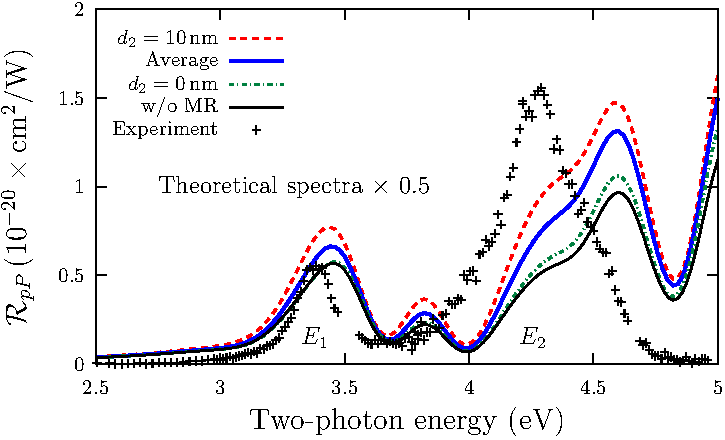
\includegraphics[width=0.48\textwidth]{fig3}
\caption{(Color online) Comparison of $\mathcal{R}_{pP}$ between the three layer
model with the effects of multiple reflections for two different values of
$d_{2}$, using the average value $\bar{R}^{M}_P$ of Eq. \eqref{eq:mcave}, the
three layer model without the effects of multiple reflections, and the
experimental data from Ref. \onlinecite{mejiaPRB02}. All curves that include
multiple reflections consider the thickness of the layer $\ell$ as $d =
10\,\mathrm{nm}$. We use $\theta = 65\,^{\circ}$, $\phi = 30\,\,^{\circ}$, and a
broadening of $\sigma = 0.075$ eV.}
\label{fig:d2values}
\end{figure}

It is important to remark that these enhancements are larger for $E_{2}$ than
for $E_{1}$. This can be understood from the fact that the corresponding
$\lambda_{0}$ for $E_{1}$ is larger than that of $E_{2}$. From Eqs.
\eqref{eq:delta0}, \eqref{eq:delta} and \eqref{mphi}, we see that the phase
shifts are larger for $E_{2}$ than for $E_{1}$, producing a larger enhancement
of the SSHG yield at $E_{2}$ from the multiple reflections. As the phase shifts
grow with $d$, so does the enhancement caused by the multiple reflections. We
have also verified that the effects of the multiple reflections from the linear
field are significantly smaller than those of the SH field. This is clear since
the phase shift of Eq. \eqref{mphi} is not only a factor of 2 smaller than that
of Eqs. \eqref{eq:delta0} and \eqref{eq:delta}, but also $w_\ell < W_\ell$. For
larger energies, such as $E_{2}$, $\lambda_{0}$ becomes smaller and the multiple
reflection effects become more noticeable. The selected value for $d <<
\lambda_{0}$, which comes naturally from the \emph{ab initio} calculation of
$\chi^{\mathrm{abc}}$, is thus very reasonable in order to model a thin surface
layer below the vacuum region where the nonlinear SH conversion takes place.

{\color{red}
Fig. \ref{fig:d2values} shows how the inclusion of multiple reflections in the
calculated SSHG yield is in better agreement with the experimental spectrum. We
can further quantify the improvement by determining the yield ratio between
$E_{2}$ and $E_{1}$ for each curve in Fig. \ref{fig:d2values}. Table
\ref{tab:rppintensity} presents these values, and we consider the maximum of
each peak for both the experimental and theoretical spectra. Using the average
value $\bar{R}^{M}_P$ yields the closest match to the experiment, while
neglecting the effects of multiple reflections has the worst peak ratio.
The addition of these effects does indeed improve the theoretical results, and
the average value for placing the nonlinear polarization would seem to be a
reasonable choice. Therefore, from this point on we will use $d=10$ nm and
$\bar{R}^{M}_{\mathrm{i}}$ from Eq. \eqref{eq:mcave} for all theoretical results
that include multiple reflections.
}

\begin{table}[b]
{\color{red}
\caption{Ratio of peak height ($E_{2}/E_{1}$) for each different curve in
Fig. \ref{fig:d2values}.}
\label{tab:rppintensity}
\centering
\begin{tabular}{ | l | c | c | }
\hline
Label                   &   $E_{2}/E_{1}$  \\
\hline
$d_{2}=10\,\mathrm{nm}$ &   1.9            \\
Average                 &   2.0            \\
$d_{2}= 0\,\mathrm{nm}$ &   1.8            \\
w/o MR                  &   1.7            \\
Experiment              &   2.8            \\
\hline
\end{tabular}
}
\end{table}

In Fig. \ref{fig:rps}, we present $\mathcal{R}_{pS}$ compared to the
experimental data; from Eq. \eqref{eq:rps111}, we can see that it is only
proportional to the $\chi^{xxx}$ component. The theoretical curve reproduces the
overall lineshape of experimental results, both in position and in intensity,
for the $E_1$ and $E_2$ resonant peaks; the resonance in between the two peaks
is slightly overestimated by the theoretical results. In this figure, we also
show the yield for the cases in which the $1\omega$ and SH multiple reflections
are neglected. We see that the overall effect in $\mathcal{R}_{pS}$ of the
$1\omega$ multiple reflections is smaller than that of the $2\omega$ multiple
reflections. As explained above, this stems from the fact of how the wavelength
$\lambda_{0}$ enters in the multiple reflection $r^{M}_p$ ($1\omega$) and
$\bar{R}^{M}_S$ ($2\omega$) factors. Of course, the full $1\omega$ and $2\omega$
multiple reflections are equally important for the SSHG yield.

\begin{figure}[t]
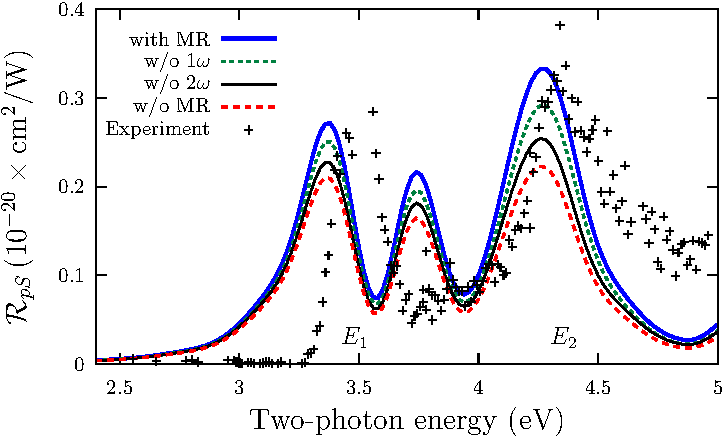
\includegraphics[width=0.48\textwidth]{fig4}
\caption{(Color online) Comparison of ${\mathcal R}_{pS}$ between the three
layer model with the full effect of multiple reflections (MR), without (w/o) the
2$\omega$ MR, without the 1$\omega$ MR, and without both 1$\omega$ and 2$\omega$
MR. All curves use the average value $\bar{R}^{M}_{s}$ and $d = 10\,\mathrm{nm}$
for the thickness of the layer $\ell$. The experimental data are taken from Ref.
\onlinecite{mejiaPRB02}. We use $\theta = 65\,^{\circ}$, $\phi =
30\,\,^{\circ}$, and a broadening of $\sigma = 0.075$ eV.}
\label{fig:rps}
\end{figure}

{\color{red}
As before, we compare the yield ratio between $E_{2}$ and $E_{1}$ for the
different spectra to determine which is closest to experiment. These values are
presented in Table \ref{tab:rpsintensity} for each curve from Fig.
\ref{fig:rps}. As before, the inclusion of the effects of multiple reflections
yields a theoretical spectra that has peak proportions closer to experiment. The
table also provides a straightforward review of how the $1\omega$ and $2\omega$
terms contribute to the peak height. Again, neglecting multiple reflections
produces the spectrum that is least similar to the experiment.
}

\begin{table}[t]
{\color{red}
\caption{Ratio of peak height ($E_{2}/E_{1}$) for each different curve in
Fig. \ref{fig:rps}.}
\label{tab:rpsintensity}
\centering
\begin{tabular}{ | l | c | c | }
\hline
Label           &   $E_{2}/E_{1}$ \\
\hline
with MR         &   1.23          \\
w/o $1\omega$   &   1.17          \\
w/o $2\omega$   &   1.12          \\
w/o MR          &   1.06          \\
Experiment      &   1.34          \\
\hline
\end{tabular}
}
\end{table}

In Fig. \ref{fig:rsp}, we present $\mathcal{R}_{sP}$ compared to the
experimental data. It is clear that the effect of the multiple reflections is
almost negligible. In the inset of the figure, we show the
$\omega^{2}\Gamma_{sP}R^{M+}_{p}$ prefactor, which comes from Eqs.
\eqref{eq:mc6}, \eqref{mcv4} and \eqref{eq:rsp111}, with and without multiple
reflections. The prefactor is almost identical in both situations, which leads
to the almost identical ${\mathcal R}_{sP}$, regardless of the effects from
multiple reflections. As we compare our calculation with the experimental data,
we see that both coincide well in position and in intensity. The experimental
$E_{1}$ and $E_{2}$ peaks have almost the same height, and this is well
reproduced in the calculated spectrum. In this case, multiple reflections do not
enhance the $E_{2}$ peak with respect to the $E_{1}$ peak, as was the case for
$\mathcal{R}_{pP}$ and $\mathcal{R}_{pS}$, further confirming the reliability of
the three-layer model.

\begin{figure}[b]
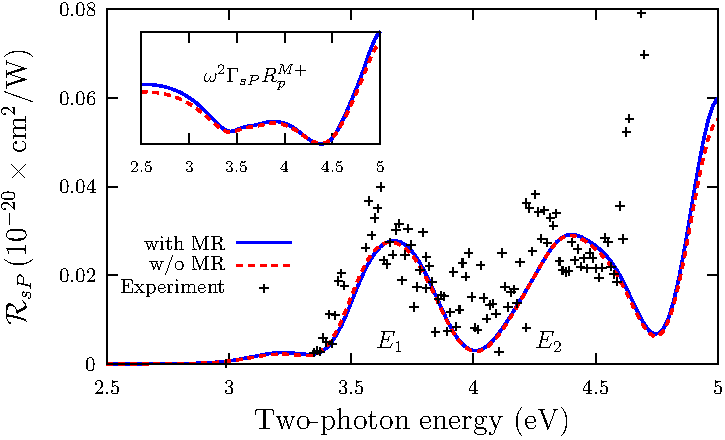
\includegraphics[width=0.48\textwidth]{fig5}
\caption{(Color online) Comparison of ${\mathcal R}_{sP}$ between the three
layer model with the full effect of multiple reflections (MR), and without (w/o)
them. The inset shows the $\omega^2\Gamma_{sP} R^{M+}_{p}$ prefactor, see text
for details. Experimental data are from Ref. \onlinecite{mejiaPRB02}. We use
$\theta = 65\,^{\circ}$, $\phi = 30\,\,^{\circ}$, and a broadening of $\sigma =
0.075$ eV.}
\label{fig:rsp}
\end{figure}


%%%%%%%%%%%%%%%%%%%%%%%%%%%%%%%%%%%%%%%%%%%%%%%%%%%%%%%%%%%%%%%%%%%%%%%%%%%%%%%%
%%%%%%%%%%%%%%%%%%%%%%%%%%%%%%%%%%%%%%%%%%%%%%%%%%%%%%%%%%%%%%%%%%%%%%%%%%%%%%%%

\section{SSHG of the
\texorpdfstring{S\lowercase{i}(001)(2$\times$1)}{Si(001)(2x1)} surface}
\label{sec:Si2x1}

The Si(001)2$\times$1 surface has electronic surface states that are ideal for
SSHG probing. Ref. \onlinecite{andersonPRB15} demonstrates how the calculation
of $\chi^{\mathrm{abc}}$ for this surface can be carried out . Here, we use a
scissors shift of $\hbar\Delta= 0.5$ eV that is the $GW$ gap reported in Refs.
\onlinecite{rohlfingPRB95} and \onlinecite{garciaCPC01}. We focus on
$\mathcal{R}_{pS}$ for which we have found that there is a very well defined
surface related SH resonant peak at a two-photon energy of 1.42 eV. The
Si(001)2$\times$1 surface reconstruction yields a Class 1 primitive triclinic
system with all the 12 components required by $\mathcal{R}_{pS}$ (Eq.
\eqref{eq:rpsmatrix}) independent from each other.\cite{popovbook} Therefore, we
cannot take advantage of any symmetry relations for this surface. However, this
is no problem for the versatile formulation we derived in Sec. \ref{sec:rcases}
which can accommodate all 12 components disregarding any surface symmetries. The
reconstruction of the Si(001)2$\times$1 surface is characterized by a dimer
along the [011] crystallographic direction that corresponds to $x$ in our
Cartesian system.\cite{andersonPRB15}

In Fig. \ref{fig:maps} we show $\mathcal{R}_{pS}$ for two different cases. In
the first, we take $\mathcal{R}_{pS}$ vs $\phi$ for a fixed $\theta_{0} =
10\,^{\circ}$, and in the second, vs $\theta_{0}$ for a fixed $\phi =
90\,^{\circ}$. We notice a very intense SSHG yield around $2\hbar\omega\sim 1.4$
eV, with less intense structures above $\sim 2.5$ eV. The former is the
surface-related SH resonance, and the latter are the resonant peaks related to
the $E_{1}$ and $E_{2}$ critical points of Si. From this figure, we see that the
best conditions for measurement are for $\phi = 90\,^{\circ}$ with a small angle
of incidence $\theta_{0}$. This azimuthal angle corresponds to incidence of the
fundamental electric field (with $p$ polarization) perpendicular to the surface
dimers, and it is quite interesting to notice that for illumination along the
dimers ($\phi = 0\,^{\circ}$ or $180\,^{\circ}$), $\mathcal{R}_{pS}\sim 0$. To
understand this behavior, we obtain from Eq. \eqref{eq:rpsmatrix} that
\begin{widetext}
\begin{equation}\label{eq:001rps90}
r_{pS}[\phi=90\,^{\circ}] =
- \left(r^{M-}_{p}\right)^{2}w^{2}_{\ell}\chi^{xyy}
- 2r^{M+}_{p}r^{M-}_{p}w_{\ell}\sin\theta_{0}\chi^{xzy}
- \left(r^{M+}_{p}\right)^{2}\sin^{2}\theta_{0}\chi^{xzz},
\end{equation}
and likewise
\begin{equation}\label{eq:001rps0}
r_{pS}[\phi=0\,^{\circ}] =
\left(r^{M-}_{p}\right)^{2}w^{2}_{\ell}\chi^{yxx}
+ 2r^{M+}_{p}r^{M-}_{p}w_{\ell}\sin\theta_{0}\chi^{yxz}
+ \left(r^{M+}_{p}\right)^{2}\sin^{2}\theta_{0}\chi^{yzz}.  
\end{equation}
\end{widetext}
The calculation of $\chi^{\mathrm{abc}}$,\cite{andersonPRB15} results in
$|\chi^{yxx}|\sim |\chi^{yxz}|\sim |\chi^{yzz}|\sim |\chi^{xzy}|<<
|\chi^{xzz}|\sim |\chi^{xyy}|$. For incoming fields along the dimers,
$\mathcal{R}_{pS}$ is very small; not because of symmetry reasons that could
cause $\chi^{yxx} = \chi^{yxz} = \chi^{yzz} = 0$, but from the electronic
structure of the surface that leads to values that are less than 1.4\,\% of the
$\chi^{xyy}$ and $\chi^{xzz}$ components involved when the incoming fields are
perpendicular to the dimers. Both, the $\phi=0^\circ$ and $\phi=90^\circ$
results can be  easily understood from the intuitive fact that the dimer is more
prone to be polarized along its length than across it.  For $\phi=0^\circ$,
$\mathcal{R}_{pS}$ involves $\chi^{y\mathrm{bc}}$ components, and the nonlinear
polarization $\boldsymbol{\mathcal{P}}$ will point only along $y$ (perpendicular
to the dimer). For $\phi=90^\circ$, the $\chi^{x\mathrm{bc}}$ components are the
ones that contribute, and these give a nonlinear polarization $\mathcal{P}^{x}$
which points along the dimer, and thus much larger than $\mathcal{P}^{y}$.
Recall that the nonlinear process mixes the direction of the exciting electric
fields with the outgoing direction of the nonlinear polarization. Therefore, we
clearly see that what is important is not the direction of excitation along or
across the dimer, but rather how the direction of the nonlinear polarization is
induced by the nonzero Cartesian components of $\chi^{\mathrm{abc}}$. This
result constitutes a clear example of what nonlinear optics is all about.

\begin{figure}[t]
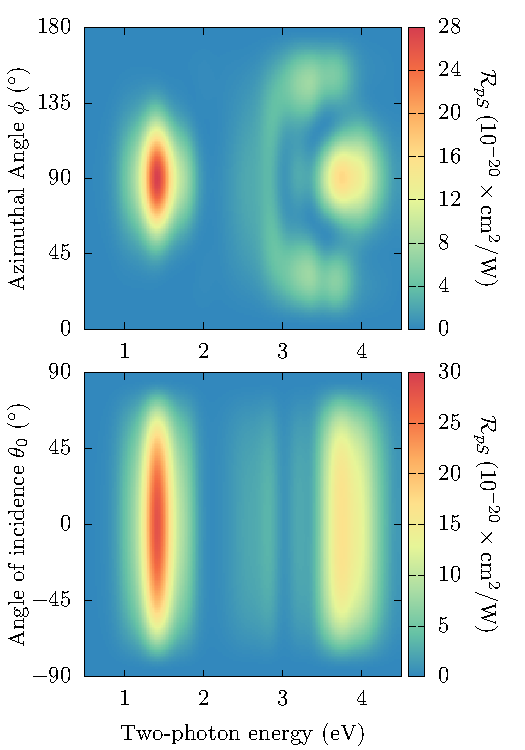
\includegraphics[width=0.48\textwidth]{fig6}
\caption{(Color online) $\mathcal{R}_{pS}$ vs two-photon energy vs $\phi$ for a
fixed $\theta = 10\,^{\circ}$ (top panel), and vs $\theta_{0}$ for a fixed $\phi
= 90\,^{\circ}$ (bottom panel), for the Si(001)(2$\times$1) surface.}
\label{fig:maps}
\end{figure}

We narrow our focus onto a particular spectrum to gain insight into these
results. In Fig. \ref{fig:rpsSi2x1} we present $\mathcal{R}_{pS}$ for $\phi =
90\,^{\circ}$ and $\theta_{0} = 10\,^{\circ}$, where we see a very well defined
surface SH peak at $2\hbar\omega = 1.42$ eV, with an intensity 17 times larger
than that of the $E_{2}$ peak for $\mathcal{R}_{pP}$ from the
Si(111)1$\times$1:H surface (see Fig.~\ref{fig:d2values}). We notice that there
are no $E_{1}$ and $E_{2}$ single peaks, but instead there is a mixture of both
resonances that produce a rather wide peak between these values. Also, we see
that the effect of multiple reflections is larger for higher energies as
discussed previously with the Si(111)1$\times$1:H surface. From the bottom panel
of the figure we see that the surface SH peak mainly comes from $\chi^{xyy}$.
The bulk SH peak is a mixture of the $\chi^{xyy}$ and $\chi^{xzz}$ components,
and $\chi^{xzy}$ is negligible. This could be geometrically interpreted as
follows. $\chi^{xyy}$ has Cartesian components only along the surface; thus, it
mainly has surface related information. On the other hand, $\chi^{xzz}$ has
``depth''($z$) components; thus, it mainly has bulk related features. Of course,
$\chi^{xyy}$ and $\chi^{xzz}$ have both bulk and surface information, which
manifests itself at the surface due to the surface's noncentrosymmetric
environment.

\begin{figure}[t]
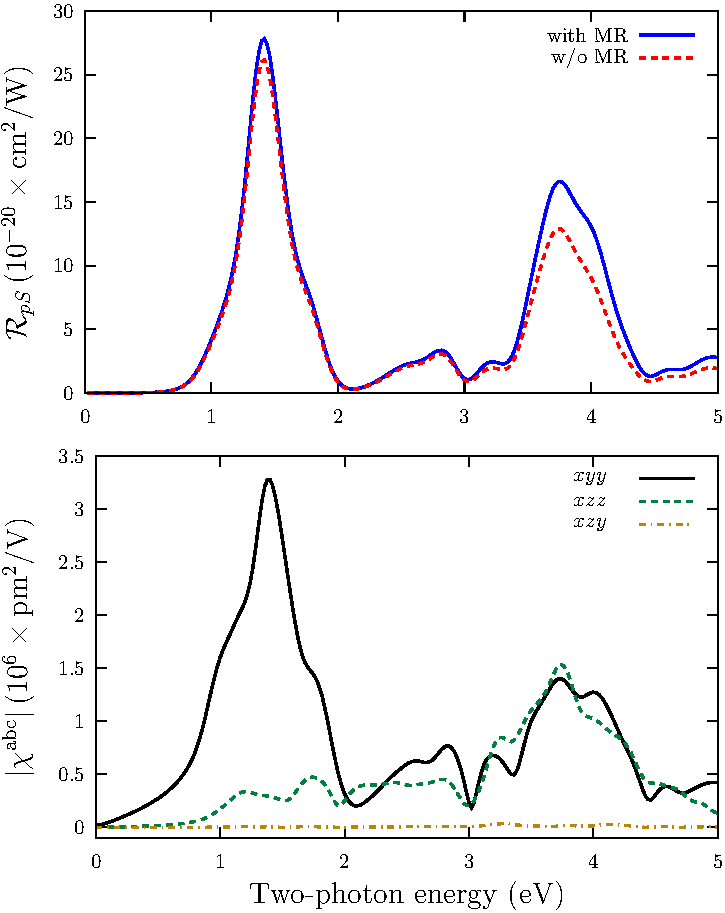
\includegraphics[width=0.48\textwidth]{fig7}
\caption{(Color online) The top panel shows, $\mathcal{R}_{pS}$ for
$\theta_{0}=10\,^{\circ}$ and $\phi=90\,^{\circ}$ for the Si(001)(2$\times$1)
surface. The bottom panel shows the components of $\chi^{\mathrm{abc}}$ involved
in $\mathcal{R}_{pS}$.}
\label{fig:rpsSi2x1}
\end{figure}

Finally, we follow Ref. \onlinecite{andersonPRB15} in order to calculate the
layer-by-layer contribution to $\chi^{xyy}$.  Each layer in the
Si(001)2$\times$1 supercell contains two Si atoms. In Fig. \ref{fig:fig8}, we
show the contribution to Im$[\chi^{xyy}]$ coming from the first (top-most) layer
that contains the dimer, the contributions from the second and third layers, and
the sum of the first eight layers. We also include
Im$[\chi^{xyy}_{\text{half-slab}}]$, that according to Ref.
\onlinecite{andersonPRB15}, is the surface value of Im$[\chi^{xyy}]$. It is this
``half-slab'' value for $\chi^{abc}$ that we use in our formulation for the SSHG
yield, presented above. As we compare against
Im$[\chi^{xyy}_{\text{half-slab}}]$, we see that Im$[\chi^{xyy}_{\text{dimer}}]$
accounts for most of the surface SH peak at 1.42 eV. The second layer also has a
small contribution to this peak. The third layer has an even smaller positive
contribution, but also a negative part that subtracts from the total peak
intensity. These negative contributions are such that as we add the first eight
layers, we obtain that Im$[\chi^{xyy}_{\text{layer 1-8}}]\sim
\text{Im}[\chi^{xyy}_{\text{half-slab}}]$; the latter includes 16 layers
(representing half of the total slab). In general, the contributions from the
different layers could have opposite signs that diminish the contribution of any
one layer towards the half-slab or surface value of $\boldsymbol{\chi}$.
Conversely, a given SH peak can be enhanced by different layers if those layers
produce contributions with the same sign. Therefore, the layer-by-layer analysis
demonstrates that the predicted SH surface peak primarily comes from the Si
dimers right at the surface of the Si(001)2$\times$1 reconstruction. This is yet
another example of the great surface sensitivity of SSHG.

\begin{figure}[b]
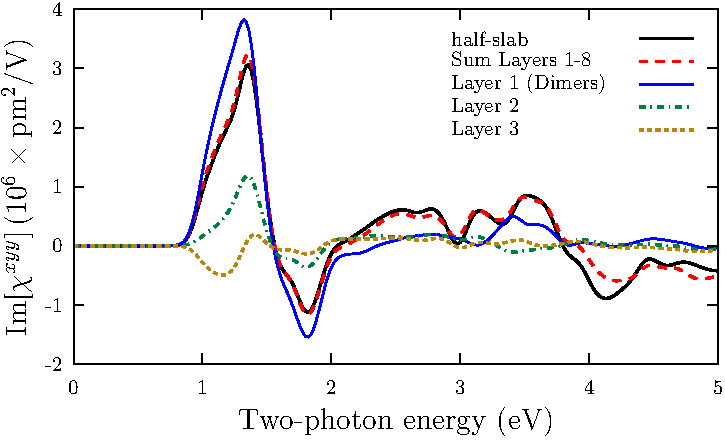
\includegraphics[width=0.48\textwidth]{fig8}
\caption{(Color online) Layer-by-layer decomposition of Im[$\chi^{xyy}$] for
the Si(001)(2$\times$1) surface (see text for details).}
\label{fig:fig8}
\end{figure}


%%%%%%%%%%%%%%%%%%%%%%%%%%%%%%%%%%%%%%%%%%%%%%%%%%%%%%%%%%%%%%%%%%%%%%%%%%%%%%%%
%%%%%%%%%%%%%%%%%%%%%%%%%%%%%%%%%%%%%%%%%%%%%%%%%%%%%%%%%%%%%%%%%%%%%%%%%%%%%%%%

\section{Conclusions}\label{sec:conclusions}

We have derived the complete expressions for the SSHG yield using the three
layer model to describe the radiating system. This treatment includes the
effects of multiple reflections inside the material from both the SH and
fundamental fields. Our derivation yields the full expressions for the yield for
the commonly used incoming and outgoing $s$ and $p$ polarizations, and can
include all the required components of $\chi^{\mathrm{abc}}$, regardless of
symmetry considerations; thus, these expressions can be applied to any surface
symmetry. We also reduce them according to the most commonly used surface
symmetries, the (111), (110) and (001) cases.

The results obtained from using the theory developed here were applied to the
Si(111)(1$\times$1):H surfaces. Our three-layer model accurately reproduces key
spectral features and yields an intensity very close to experiment for all the
cases studied. We consider it an upgrade over the much reviewed two layer
model,\cite{mizrahiJOSA88} and it comes with very little added computational
expense. The addition of the effects of multiple reflections either enhances the
intensity of the calculated spectra and improves the peak proportions, or has
little effect at all, always in close agreement with experiment.

We also presented a predictive study of the SSHG yield from Si(001)(2$\times$1)
surface. As mentioned above, our robust formulation can accomodate all 18
independent components (for SHG) of $\chi^{\mathrm{abc}}$ for any surface, and
we focused on $\mathcal{R}_{pS}$ which uses 12 of these components. We find
clear evidence of electronic surface states around a two-photon energy of 1.41
eV, and we present a brief overview of the produced SSHG yield over a wide range
of incident ($\theta_{0}$) and azimuthal ($\phi$) angles, along with a physical
understanding of the results. This type of plots will be quite useful to the
experimentalist interested in this kind of spectroscopy. Overall, our
theoretical three-layer model can be used to quantitatively study the SSHG
yield.


%%%%%%%%%%%%%%%%%%%%%%%%%%%%%%%%%%%%%%%%%%%%%%%%%%%%%%%%%%%%%%%%%%%%%%%%%%%%%%%%
%%%%%%%%%%%%%%%%%%%%%%%%%%%%%%%%%%%%%%%%%%%%%%%%%%%%%%%%%%%%%%%%%%%%%%%%%%%%%%%%


\section{Acknowledgements}\label{sec:acknowledgements}

B.S.M. acknowledges partial support from CONACYT-M\'exico Grant 153930. S.M.A.
gratefully acknowledges full support from CONACYT-M\'exico scholarship 349278.

\bibliographystyle{unsrt}

\begin{thebibliography}{10}

\bibitem{chenPRL81}
C.~K. Chen, A.~R.~B. de~Castro, and Y.~R. Shen.
\newblock Surface-enhanced second-harmonic generation.
\newblock {\em Phys. Rev. Lett.}, 46(2):145--148, January 1981.

\bibitem{shenNAT89}
Y.~R. Shen.
\newblock Surface properties probed by second-harmonic and sum-frequency
  generation.
\newblock {\em Nature}, 337(6207):519--525, February 1989.

\bibitem{mcgilpOE94}
J.~F. McGilp, M.~Cavanagh, J.~R. Power, and J.~D. O'Mahony.
\newblock Probing semiconductor interfaces using nonlinear optical
  spectroscopy.
\newblock {\em Opt. Eng.}, 33(12):3895--3900, 1994.

\bibitem{bloembergenAPB99}
N.~Bloembergen.
\newblock Surface nonlinear optics: a historical overview.
\newblock {\em Appl. Phys. B-Lasers O.}, 68(3):289--293, 1999.

\bibitem{mcgilpSRL99}
J.~F. McGilp.
\newblock Second-harmonic generation at semiconductor and metal surfaces.
\newblock {\em Surf. Rev. Lett.}, 6(03n04):529--558, 1999.

\bibitem{lupkeSSR99}
G.~L{\"u}pke.
\newblock Characterization of semiconductor interfaces by second-harmonic
  generation.
\newblock {\em Surf. Sci. Rep.}, 35(3):75--161, 1999.

\bibitem{downerPSSA01}
M.~C. Downer, Y.~Jiang, D.~Lim, L.~Mantese, P.~T. Wilson, B.~S. Mendoza, and
  V.I. Gavrilenko.
\newblock Optical second harmonic spectroscopy of silicon surfaces, interfaces
  and nanocrystals.
\newblock {\em Phys. Status Solidi A}, 188(4):1371--1381, 2001.

\bibitem{downerSIA01}
M.~C. Downer, B.~S. Mendoza, and V.~I. Gavrilenko.
\newblock Optical second harmonic spectroscopy of semiconductor surfaces:
  advances in microscopic understanding.
\newblock {\em Surf. Interface Anal.}, 31(10):966--986, 2001.

\bibitem{vanhasseltJOSAB95}
C.~W.~van Hasselt, M.~A.~C. Devillers, Th. Rasing, and O.~A. Aktsipetrov.
\newblock Second-harmonic generation from thick thermal oxides on {Si}(111):
  the influence of multiple reflections.
\newblock {\em J. Opt. Soc. Am. B}, 12(1):33, January 1995.

\bibitem{kolthammerPRB05}
William~S. Kolthammer, Dustin Barnard, Nicole Carlson, Aaron~D. Edens,
  Nathan~A. Miller, and Peter~N. Saeta.
\newblock Harmonic generation in thin films and multilayers.
\newblock {\em Phys. Rev. B}, 72(4):045446, July 2005.

\bibitem{yeganehPRB92}
M.~S. Yeganeh, J.~Qi, J.~P. Culver, A.~G. Yodh, and M.~C. Tamargo.
\newblock Interference in reflected second-harmonic generation from thin
  nonlinear films.
\newblock {\em Phys. Rev. B}, 46(3):1603--1610, July 1992.

\bibitem{haseAPL92}
Y.~Hase, K.~Kumata, S.~S. Kano, M.~Ohashi, T.~Kondo, R.~Ito, and Y.~Shiraki.
\newblock New method for determining the nonlinear optical coefficients of thin
  films.
\newblock {\em Appl. Phys. Lett.}, 61(2):145--146, 1992.

\bibitem{buinitskayaMJPS02}
G.~Buinitskaya, I.~Kravetsky, L.~Kulyuk, V.~Mirovitskii, and E.~Rusu.
\newblock Optical {Second} {Harmonic} {Generation} {In} {ZnO} {Film}:
  {Multiple}-reflection {Effects}.
\newblock {\em Moldavian Journal of the Physical Sciences}, 1(N4), 2002.

\bibitem{buinitskayaCAS03}
G.~Buinitskaya, I.~Kravetsky, L.~Kulyuk, V.~Mirovitskii, and E.~Rusu.
\newblock Characterization of thin {ZnO} film by optical second harmonic
  generation: experiment and theory.
\newblock In {\em Semiconductor Conference, 2003. CAS 2003. International},
  volume~2, page 322, September 2003.

\bibitem{makerPRL62}
P.~D. Maker, R.~W. Terhune, M.~Nisenoff, and C.~M. Savage.
\newblock Effects of {Dispersion} and {Focusing} on the {Production} of
  {Optical} {Harmonics}.
\newblock {\em Phys. Rev. Lett.}, 8(1):21--22, January 1962.

\bibitem{tellierOC07}
G.~Tellier and C.~Boisrobert.
\newblock Second harmonic generation: {Effects} of the multiple reflections of
  the fundamental and the second harmonic waves on the {Maker} fringes.
\newblock {\em Optics Communications}, 279(1):183--195, November 2007.

\bibitem{abeJOSAB08}
M.~Abe, I.~Shoji, J.~Suda, and T.~Kondo.
\newblock Comprehensive analysis of multiple-reflection effects on rotational
  {Maker}-fringe experiments.
\newblock {\em J. Opt. Soc. Am. B}, 25(10):1616, October 2008.

\bibitem{bloembergenPR62}
N.~Bloembergen and P.~S. Pershan.
\newblock Light {Waves} at the {Boundary} of {Nonlinear} {Media}.
\newblock {\em Physical Review}, 128(2):606--622, October 1962.

\bibitem{dickAPB85}
B.~Dick, A.~Gierulski, G.~Marowsky, and G.~A. Reider.
\newblock Determination of the nonlinear optical susceptibility $\chi^{(2)}$ of
  surface layers by sum and difference frequency generation in reflection and
  transmission.
\newblock {\em Appl. Phys. B}, 38(2):107--116, October 1985.

\bibitem{sipePRB87}
J.~E. Sipe, D.~J. Moss, and H.~M. van Driel.
\newblock Phenomenological theory of optical second- and third-harmonic
  generation from cubic centrosymmetric crystals.
\newblock {\em Phys. Rev. B}, 35(3):1129--1141, January 1987.

\bibitem{mizrahiJOSA88}
V.~Mizrahi and J.~E. Sipe.
\newblock Phenomenological treatment of surface second-harmonic generation.
\newblock {\em J. Opt. Soc. Am. B}, 5(3):660--667, 1988.

\bibitem{ciniPRB91}
Michele Cini.
\newblock Simple model of electric-dipole second-harmonic generation from
  interfaces.
\newblock {\em Phys. Rev. B}, 43(6):4792--4802, February 1991.

\bibitem{moritaJJAP88}
Ryuji Morita, Takashi Kondo, Yushi Kaneda, Atsushi Sugihashi, Nagaatsu
  Ogasawara, Shinsuke Umegaki, and Ryoichi Ito.
\newblock Multiple-{Reflection} {Effects} in {Optical} {Second}-{Harmonic}
  {Generation}.
\newblock {\em Japanese Journal of Applied Physics}, 27(Part 2, No.
  6):L1134--L1136, June 1988.

\bibitem{goosAP47}
F.~Goos and H.~H\"anchen.
\newblock Ein neuer und fundamentaler {Versuch} zur {Totalreflexion}.
\newblock {\em Ann. Phys.}, 436(7-8):333--346, January 1947.

\bibitem{shihPRA71}
H.~Shih and N.~Bloembergen.
\newblock Phase-{Matched} {Critical} {Total} {Reflection} and the
  {Goos}-{Haenchen} {Shift} in {Second}-{Harmonic} {Generation}.
\newblock {\em Phys. Rev. A}, 3(1):412--420, January 1971.

\bibitem{yallapragadaSR16}
Venkata~Jayasurya Yallapragada, Ajith~P. Ravishankar, Gajendra~L. Mulay,
  Girish~S. Agarwal, and Venu~Gopal Achanta.
\newblock Observation of giant {Goos}-{H\"anchen} and angular shifts at
  designed metasurfaces.
\newblock {\em Sci. Rep.}, 6:19319, January 2016.

\bibitem{yallapragadaOE13}
V.~J. Yallapragada, Achanta~Venu Gopal, and G.~S. Agarwal.
\newblock Goos-{H\"anchen} shifts in harmonic generation from metals.
\newblock {\em Opt. Express}, 21(9):10878, May 2013.

\bibitem{reiningPRB94}
L.~Reining, R.~Del~Sole, M.~Cini, and J.~G. Ping.
\newblock Microscopic calculation of second-harmonic generation at
  semiconductor surfaces: {As/Si(111)} as a test case.
\newblock {\em Phys. Rev. B}, 50(12):8411--8422, 1994.

\bibitem{andersonPRB15}
S.~M. Anderson, N.~Tancogne-Dejean, B.~S. Mendoza, and V.~V{\'e}niard.
\newblock Theory of surface second-harmonic generation for semiconductors
  including effects of nonlocal operators.
\newblock {\em Phys. Rev. B}, 91(7):075302, February 2015.

\bibitem{andersonPRB16}
S.~M. Anderson, N.~Tancogne-Dejean, B.~S. Mendoza, and V.~V{\'e}\-niard.
\newblock Improved \emph{ab initio} calculation of surface second-harmonic
  generation from si(111)(1{$\times$}1)h.
\newblock {\em Phys. Rev. B}, 93(23):235304, May 2016.

\bibitem{mejiaRMF04}
J.~E. Mej{\'i}a, B.~S. Mendoza, and C.~Salazar.
\newblock Layer-by-layer analysis of second harmonic generation at a simple
  surface.
\newblock {\em Revista Mexicana de F\'{\i}sica}, 50(2):134--139, 2004.

\bibitem{mejiaPRB02}
J.~E. Mej{\'i}a, B.~S. Mendoza, M.~Palummo, G.~Onida, R.~Del~Sole, S.~Bergfeld,
  and W.~Daum.
\newblock Surface second-harmonic generation from si (111)(1x1) h: Theory
  versus experiment.
\newblock {\em Phys. Rev. B}, 66(19):195329, 2002.

\bibitem{aktsipetrovJETP86}
A.~Aktsipetrov, I.~M. Baranova, and A.~Il'inskii.
\newblock Surface contribution to the generation of reflected second-harmonic
  light for centrosymmetric semiconductors.
\newblock {\em J. Exp. Theor. Phys.}, 64(1):167, 1986.

\bibitem{xuJVST97}
Z.~Xu, X.~F. Hu, D.~Lim, J.~G. Ekerdt, and M.~C. Downer.
\newblock Second harmonic spectroscopy of {Si}(001) surfaces: {Sensitivity} to
  surface hydrogen and doping, and applications to kinetic measurements.
\newblock {\em J. Vac. Sci. Technol. B}, 15(4):1059--1064, July 1997.

\bibitem{guyotPRB88}
P.~Guyot-Sionnest and Y.~R. Shen.
\newblock Bulk contribution in surface second-harmonic generation.
\newblock {\em Phys. Rev. B}, 38(12):7985--7989, October 1988.

\bibitem{shenAPB99}
Y.~R. Shen.
\newblock Surface contribution versus bulk contribution in surface nonlinear
  optical spectroscopy.
\newblock {\em Appl. Phys. B}, 68(3):295--300, 1999.

\bibitem{boyd}
R.W. Boyd.
\newblock {\em Nonlinear Optics}.
\newblock Academic Press, New York, 2003.

\bibitem{sutherland}
Richard~L. Sutherland.
\newblock {\em Handbook of {Nonlinear} {Optics}}.
\newblock CRC Press, April 2003.

\bibitem{sipeJOSAB87}
J.~E. Sipe.
\newblock New {Green}-function formalism for surface optics.
\newblock {\em Journal of the Optical Society of America B}, 4(4):481--489,
  1987.

\bibitem{jacksonbook}
J.~D. Jackson.
\newblock {\em Classical Electrodynamics, 3rd Edition}.
\newblock Wiley-VCH, 3rd edition edition, July 1998.

\bibitem{andersonPHD16}
S.~M. Anderson.
\newblock {\em Theoretical Optical Second-Harmonic Calculations for Surfaces}.
\newblock PhD thesis, Centro de Investigaciones en \'Optica, A.C., July 2016.

\bibitem{mitchellSS01}
S.~A. Mitchell, M.~Mehendale, D.~M. Villeneuve, and R.~Boukherroub.
\newblock Second harmonic generation spectroscopy of chemically modified {Si}(1
  1 1) surfaces.
\newblock {\em Surf. Sci.}, 488(3):367--378, August 2001.

\bibitem{bergfeldPRL04}
S.~Bergfeld, B.~Braunschweig, and W.~Daum.
\newblock Nonlinear {Optical} {Spectroscopy} of {Suboxides} at {Oxidized}
  {Si}(111) {Interfaces}.
\newblock {\em Phys. Rev. Lett.}, 93(9):097402, August 2004.

\bibitem{liPRB10}
Y.~Li and G.~Galli.
\newblock Electronic and spectroscopic properties of the hydrogen-terminated
  {Si}(111) surface from ab initio calculations.
\newblock {\em Phys. Rev. B}, 82(4):045321, July 2010.

\bibitem{yubook}
P.~Yu and M.~Cardona.
\newblock {\em Fundamentals of {Semiconductors}: {Physics} and {Materials}
  {Properties}}.
\newblock Springer Science \& Business Media, third edition, March 2005.

\bibitem{rohlfingPRB95}
M.~Rohlfing, P.~Kr{\"u}ger, and J.~Pollmann.
\newblock Efficient scheme for {GW} quasiparticle band-structure calculations
  with applications to bulk si and to the si(001)-(2x1) surface.
\newblock {\em Phys. Rev. B}, 52(3):1905--1917, July 1995.

\bibitem{garciaCPC01}
P.~Garc{\'i}a-Gonz{\'a}lez and R.~W. Godby.
\newblock {GW} self-energy calculations for surfaces and interfaces.
\newblock {\em Comput. Phys. Commun.}, 137(1):108--122, June 2001.

\bibitem{popovbook}
S.~V. Popov, Y.~P. Svirko, and N.~I. Zheludev.
\newblock {\em Susceptibility tensors for nonlinear optics}.
\newblock CRC Press, 1995.

\end{thebibliography}
\end{document}